\documentclass{article}
\usepackage{enumitem}
\usepackage[utf8]{inputenc}
\usepackage{graphicx} 
\usepackage{epstopdf}
\begin{document}
\author{Frederik Laboyrie}
\title{Multiresolution Convolutional Neural Network Architectures for Hand Orientation Inference}
\maketitle
\begin{abstract}
\emph{In this work an efficient convolutional neural network (CNN) architecture will be developed which is capable of inferring hand orientation angle through regression on uncalibrated 2D monocular images. This is a useful technique in augumented reality and human computer interaction which often rely on low resource hardware such as handheld mobile devices which have slower processing speed and lack depth sensors.}
\end{abstract}

\pagebreak


\section{Introduction}
\subsection{Introduction and Objectives}

In this work an efficient convolutional neural network (CNN) architecture will be developed which is capable of inferring hand orientation angle through regression on uncalibrated 2D monocular images. This is a useful technique in augumented reality and human computer interaction which often rely on low resource hardware such as handheld mobile devices which have slower processing speed and lack depth sensors.\\

\vspace*{-4mm}
\begin{figure}[h]
  \centering
  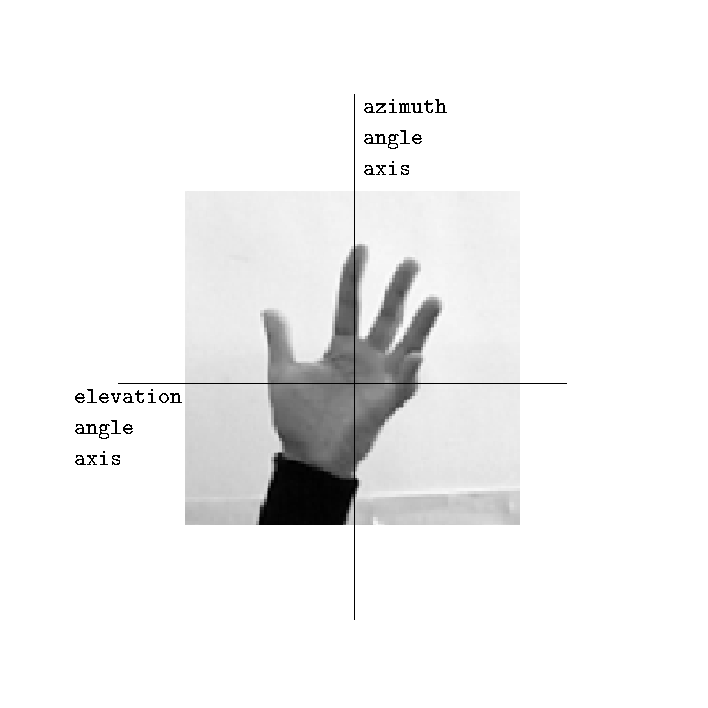
\includegraphics[scale=0.8]{example_hand2.pdf}
  \vspace*{-10mm}
  \caption{An example input image and corresponding angle axes}
  \label{fig:example_hand}
\end{figure}

An example image a hand which is provided as input during the training process in this work is shown in figure \ref{fig:example_hand}. The azimuth and elevation angles then describe the orientation of a hand in any given image. \\

This task specifically builds on the work in [17] where manually extracted contour distance features were used to train a multi-layered Random Forest (ML-RF hereafter). I will apply techniques more related to state-of-the-art performance in hand pose estimation which typically use complex Convolutional Neural Network (CNN hereafter) architectures. CNNs are capable of automatically extracting features during the training process and are widely used to achieve state-of-the-art performance in many computer vision tasks. \\

However, many challenges have plagued this task due to the complicated nature of hands. For instance natural self occlusion, extreme similarity in the appearance of certain orientations and the necessity to be able to model from a wide variety of view points for approaches to be useful in real life situations. This makes it for models to pick up on small differences and to understand how differing shapes of a hand may not affect orientation. Other challenges such as high joint flexibility are specific to architectures where joints may be modelled on individually. \\

It is largely for these reasons that complex architectures, such as those which focus on joints, as previously mentioned, but also those which take multiple inputs of varying resolutions in order to build a wider variety of features to aid the training process. Complex network architectures such as these do not lend well to low resource hardware as producing output becomes much more costly. Tasks such as hand orientation inference and hand pose estimation generally will be taking place in real time and the latency of a model is of concern along with accuracy. \\

For this reason, my objective in this work is not only to develop network architectures inspired by recent advances in hand-related tasks but also to experiment with variations in these architectures which decrease latency. These variations will be driven by using alternatives to standard convolutional filters, which make up the mechanism through which CNNs extract features from pixel values. In this work, SqueezeNets [8] and MobileNets [1] will be used to provide architectural variations and will be evaluated on whether they can match the performance of a standard CNN.\\

I will be using an identical dataset as was used in [17], so I will be able to benchmark my results to those gained in [17]. It is therefore my aim to improve on the accuracy in [17], or at least match it if the resulting architecture used to gain results is amenable to low resource hardware. In this way, it also my aim for the standard CNNs performance to be matched by the performance of SqueezeNets [8] and MobileNets[1], the architectures developed for low resource hardware. \\

It is a well known result for low latency architectures to have little to no loss in performance, but it is not known whether they are suitable for this intricate task as any spatial information being lost during the convolutions could potentially have large effects on the final accuracy.Nevertheless,it is worth highlighting that the primary challenge in this task will be able to build any architecture capable of picking up on the intricate spatial relations of hand positions rather than replicating a well known result of low latency networks not causing significant loss in performance. \\

If successful, potential beneficiaries of the resulting models would be augmented reality and virtual reality developers for applications which aim to be viable to run on a wide array of hardware. The decrease computational complexity of these models compared to those achieving state-of-the-art accuracy, would allow them to utilise texture features extracted by convolutional filters, ideally increasing accuracy with neglibile loss in latency compared to ML-RF approaches. Then applications could be developed which could more easily project 3D images onto hands, or develop games which use the orientation of a hand to control the game environment.\\

As at the time of writing, newer high-end mobile devices tend to be built with binocular cameras or stand-alone depth sensors architectures. However, any model architectures put forward in this work could equally be trained using depth values in addition to RGB values or even training on depth values alone. It is therefore not necessary to discount the possibility of using these architectures on devices which are capable of deriving depth information. \\

The dataset was collected by the Computer Vision group at City, University of London and as of yet has not had these techniques applied to it. In this way, the group are also potential beneficiaries of this work if the results are more promising than those gained in the first work [17] to use them.\\

The desired outcome of this work are the results alone and I do not plan within this work to experiment with the resulting models integration into a product. Analysis of the results will of course take use cases of the models into account. For example, by favouring low variance in error or understanding whether any improvements in error are worth the potential increases in latency.  \\

I also want to highlight the specific goals of this work are similar to those in [17]. The focus is on developing a generalizable technique in which hand orientation can be inferred from multiple viewpoints on any hand in a quick manner, that is one which does not require calibration. This process is used to estimate the parameters of a lens which can allow objects to be measured accurately in a 3D scene. It is a lengthy process and inappropriate for developing a model which can work over a variety of hardware.\\

\subsection{Changes Since Proposal}
The modelling techniques used in this work were not ones originally proposed. The models used in this work are more suited to the task at hand as they are generally suitable for low resource hardware. The proposal to use knowledge distillation and HashedNets was in fact far less appropriate than the usage of SqueezeNets and MobileNets, for reasons explain in Sections 2.2.2 and 2.2.3 respectively.

\section{Critical Context}
This work not only takes into account work specifically around hand-related tasks but also work which can be more generally applied to machine learning tasks. These will both be discussed in this section and techniques chosen to be applied will be discussed in detail in the following section.   

\subsection{Hand Pose and Orientation Inference}
Hand pose and orientation inference tasks can be performed both in a discriminative and a generative manner. Discriminative approaches are capable of providing an output of angle or pose for any given image once a model is built using only a single frame. Generative approaches rather build, as an intermediate representation, a model of the hand from which orientation can be inferred following initialisation.\\

Building discriminative models for hand pose and orientation inference is a task which typically requires non-standard architectures due to its intricacy. Training capacity must be used to model very small changes and it is often useful to use more global features. For example with hand orientation, global features can be used to dismiss large parts of angle space and then local features are learnt in conjunction with these and can potentially provide additional accuracy as the features can become specific to areas in angle spaces. Without the use of global features the localized features would have to infer all information about the hand but may be insufficient to provide discriminative power\\

This technique is used in [13] where a multiresolution CNN is used on a dataset of RGBD images for real time pose-recovery. A 96x96 image is downsampled 2x and 4x, where the more downsampled an image the more global the features can be extracted. The features are more global as a filter of a given size will convolve over a larger space over a low resolution image compared to a high resolution and therefore outputs more general information about the shape of the hand. The images of differing resolutions are passed into separate CNNs before their feature maps are flattened, concatenated and passed into fully-connected layers. It would of course be an alternative to use larger filters instead of downsampling but this increases learning capacity and requires significantly more computation both during training and at runtime.\\

In [13] the network does not simply trained on a label but is trained to generate 14 18x18 heatmaps which represent the probability of a given joint being in a location. These heatmaps are then combined using the inverse kinematics algorithm to recover the pose of the hand. Note that the training is compartmentalised into 14 separate heatmaps each representing a separate joint, rather than learning the location of all joints individually. These intermediate heatmaps allow the network to focus on local features which increases accuracy. It also allows better recovery of pose if a heatmap fails as the other non-failing heatmaps can be used with a heuristic.\\

[13] is not unique in using joint angle and position for solving hand pose estimation. [14], for example directly estimates 3D joint location with a variety of architectures including, multi-scale, deep and shallow. In [14], as well, the physical constraints of joint positions in a hand are also used in alternate architecture which models first a low dimensional embedding. This lower implicit dimensionality forces the network to learn whilst the physical constraints of the hands are enforced. There is an additional reconstruction layer which projects the lower dimensional vector back into higher dimensional joint space. In this way, it still models the joint locations directly, but the low dimensional embedding before the reprojection acts as a 'bottleneck', restricting training. [14] goes further in a refining stage where a separate network is used for each joint along with a system which corrects overlapping regions.\\

[15], by the same authors as in [14], again estimates 3D joint location but uses these locations to develop synthesised images of hands. Synthesised images of hands using poorly estimated 3D joint location will result in an image which does not well represent a hand and will be malformed in shape. For refinement, something similar to a Siamese network is then used in [15]. This network is a multi-input network with a weight constraint in each path such that both paths have identical weights before their output is concatenated before being passed into shared fully-connected layer.\\

This network has the synthesised image and the true image passed into the Siamese network architecture which iteratively updates the 3D joint location to reduce disparity between the synthesised image and the true image which leads to more accurate 3D joint location estimation. To increase the speed of this convergence a given factor between 0 and 1 is used as a minimal improvement along with Gaussian noise being applied to the poses which allows the synthesised image to converge more quickly to the true image.\\

[16] uses fully 3D information, noting that in [13] the joint location probability heat maps which are the results of the regression only contain 2D information. This is done by modelling on multiple views which are obtained by projecting the original single-depth images onto three orthogonal planes. Because the 2D positions of the joints are projected onto multiple planes, multiple-view CNNs are then more robust to errors in 2D location estimation which could results in large depth estimation errors in single-view CNNs. They are also more robust to ambiguity and can learn hand constraints implicitly as opposed to it being pre-defined as in [13]. This technique was able to achieve state-of-the-art results on multiple datasets including ones which originally relied on calibration and tracking rather than being purely data-driven.\\

This work will focus exclusively on hand orientation on 2D uncalibrated monocular images and will follow on from work in [17] where azimuth and elevation axis angles are modelled on directly. I will continue this approach of modelling directly on the images and the labels. Further, as the dataset in [17] provides labels for the angles and not for joint location, it is far from trivial to integrate anything beyond broader architectural choices from the previous existing body of work. Most feasible, is the multi-input architecture which I believe is a significant enough step up in complexity from the ML-RF approach to form a basis for this work as it is an underlying similarity that exists in recent work in this area. \\

Further, modelling on joint locations is intuitively something that is much more important for hand pose estimation. In hand orientation in general, and specifically in [17], the hand is seen in a similar position so it is not necessary to infer the hand orientation from joint position but rather it can be inferred directly.\\

The combination of global and local features intends to replace certain characterteristics that derive from [17]'s best results which are achieved using a ensemble of expert regressors which each focus on a particular area of angle space.  In order to allow for this, [17]'s architecture includes a first layer which outputs the posterior probality of a given example belonging to a particular part of angle space. This of course allows the model to dismiss large regions of angle space and gain benefit from the expert regressors. Note that all of the regressors in [17] are Random Forests which use contour distance features as input. \\

[17] develops a method in which each expert regressor will output a posterior probability of an example belonging to its subspace. However, instead of using these posterior probabilities naively, during training the ground truth probabilities are used alongside the expert regressor's posterior probabilities to learn a marginalised probability distribution from which the marginalised regressors weights are derived from. Essentially, this is learning a way to combine the  posterior probabilites to form a marginalised probability distribution most similar to the ground truth probability. This was done using a novel optimisation technique similar to  Kullback-Leibler divergence [31]. \\

[17] using a marginalisation layer followed by expert regressors would make their approach a multi-layer Random Forest (ML-RF hereafter). Whereas [17] developed a novel and generalizable technique as previously described, a significant body of work exists also utilising ML-RF for similar tasks. [18] uses an ML-RF but for hand-pose estimation. The first layer classifies a general shape and the second layer focuses on classifying particular parts of the hand. [18] most noticeably differs from [17] in that the posterior probabilities are used naively and are simply used to weight the posterior probabilities of the second layer. They are not used to model a marginal probability during training. \\

Note that combining these posterior probabilities in this context has a similar effect to the way that the concatentated feature maps in multi-input map are modelled on simultaneously in the final layers of the network. This is in that the models are training on several sources of information which are describing separate things. In the context of the multi-input architectures the combination of global and local features serve the same purpose. It would be possible to further train expert networks but this would increase computaional complexity greatly and limit the effect of any improvement in convolutional latency. \\

ML-RF techniques are computationally cheap and able to achieve acceptable performance but Random Forests are not able to build complex combined features as CNNs are able to. These features allow much greater accuracy and can model on the hand directly whereas Random Forests must rely on extracted features as well. Modelling on the pixels directly also allow CNNs to obtain information on non-contour pixels which can contain information such as shading. Further, extracted features, specifically contour distance features, need precise segmentation in order to be accurate and so can be difficult to compute robustly. \\

 CNNs consistently achieve state-of-the-art on this task undoubtedly due to these advantages. Vanilla CNNs are extremely costly computationally both during training and run-time. However, recent advances (described in following section) have drastically reduced the cost and size of CNNs with minimal to no loss in computational accuracy. This makes them potentially suitable for this task in real-time. \\

It is important to note that despite complex CNN architectures achieving state of the art performance in many hand pose or orientation estimation tasts, the gains are not significant over Random Forest methods. A reason noted in [20] is that the CNNs architectures than have emerged are relatively shallow compared to those where achieve state of the art on other tasks such as ImageNet [32]. This is partly due to avoid overfitting on small datasets such as the one that will be used in this task. \\

Note that the generative techniques in [21, 25] are for dataset generation or augmentation and remain completely separate from previous work which uses generative techniques to infer hand pose directly. These more typical modern generative techniques are largely based around building a 3D model of the hand and tracking the individual components of the model in real-time in order to infer the pose. This was done  in [26] where a hand model  where the hand model was build using geometric primitives.\\

These generative techniques typically rely on strong computational power with multi-GPU set ups and typically fail to generalize on a new user's hand which cause them to be completely separate to what is aiming to be achieved in this work. Generative techniques also suffer from drift, that is accumulation of errors, which was confronted in [21] using local adversarial loss.\\ 

In [20], several best practices are explored whilst using an Regional Ensemble Net architecture, which similarly to other. architectures models directly on 3D hand joint co-ordinates. The Regional Ensemble Net architecture produces feature maps which focus on different regions of the image. These region wise feature maps are concatenated and passed into fully-connected layers where they can combine into complex joint features. Concatenating these feature maps rather than using average pooling across the feature maps was shown to improve performance again as the network can learn itself how best to combine them. [20] is unique in that different views of inputs are used simultaneously during training to predict the same pose, rather than just during testing to check robustness. \\

[20] is another example of concatenation of feature maps from differing networks, as opposed to any other aggregation method. This makes concatenation a clear choice for models in this work. The regional aspect of [20] is largely useful for pose estimation where regions of the hand may differ largely between poses. Although this is largely driven by intuition, I did not choose to experiment with it as it is non-trivial to implement and without obvious benefits. \\

\subsection{Memory Overhead Management}
Reducing network latency and size largely falls into two categories, those are taking measures in the initial structure of the network and those which are applied after training. Most techniques are both applicable to making smaller networks suitable for low resource hardware as well as making much larger networks capable of fitting on GPUs in order to take advantage of parallel processing.

\subsubsection{Managing Network Memory Usage via Initial Structure}

Traditional CNNs, despite their ability in achieving high accuracy on many tasks, have several computational inefficiencies that are more apparent when developing large models or relying on low resource hardware. These inefficiencies  arise both from their spatial convolutions and CNNs' typical reliance on many fully-connected layers at the top of the network which often contain the vast majority of the parameters. In developing efficient networks, both in terms of latency and size, it is possible to work around these inefficiencies in many ways. Specifically, in terms of initial structure, this means replacing standard convolutions with more efficient convolutions.\\

MobileNets [1] utilize depthwise separable convolutions which are efficient both in terms of latency  and number of parameters. These are factorized convolutions in which depthwise convolutions are performed separately on each input channel. These are then followed by 1x1 pointwise convolutions on each feature map and only then are outputs combined. A more detailed description of these convolutions in in section 3.\\ 

By separating these stages computational cost is reduced 8-9x when using 3x3 depthwise separable convolutions as in [1]. [2] notes that separating depthwise and pointwise convolutions also prevents a single convolutional kernel having to map spatial correlations and cross-channel correlations jointly. Depthwise separable convolutions are utilised heavily in very deep architectures focused on achieving state-of-the-art results [2, 10]. MobileNets [1], however, utilise them for their efficiency. \\

MobileNets have a base structure which is then controlled by model-shrinking parameters. One parameter alters the width of each layer in the network uniformly and the other is a resolution multiplier. Note that both of these parameters are only used to parametrise a new structure which must be trained again. They primarily exist to provide ease of use for developers aiming to optimise the cost of their network.\\

The utilisation of 1x1 convolutions in MobileNets is not unique to that architecture and are generally popular in model architectures motivated by low latency and model size. SqueezeNets [8] use them not only for the fewer parameters but also to reduce the number of input channels. This is done in Fire modules which replace the convolutional layers. Fire modules have a squeeze layers within them which utilise 1x1 convolutions to greatly restrict the number of input channels being pased to the expand layer. Fire modules are then much more parameter efficient than standard convolutional layers and are described in more detail in Section 3. SqueezeNets also delay downsampling until later in the network rather than having to downsample each layer with pooling which is shown to increase classification accuracy in [9].\\

SqueezeNets are in fact fully convolutional which further reduces parameters by avoiding the large number of weights which fully-connected layers introduce. Despite this, the model size can still be reduced considerably, well above 50x in terms of parameters, using Deep Compression  [11] and still not lose classification accuracy.\\

SqueezeNets and MobileNets are then extremely suitable for this particular task. It is clearly shown in  literature that it is possible to build much more efficient models without losing accuracy, making these models suitable for low-resource hardware and therefore chosen as alternate architectures to those provided by standard CNNs. \\
\subsubsection{Compressing Models After Training}

Deep Compression is a procedure of several stages which allows compression of models 35-50x without loss of accuracy. This allows extremely large models to still fit on embedded devices. Although the focus is largely on model size, latency can be lowered if the model is reduced enough in size to avoid having to store it in off-chip DRAM memory and can be stored in on-chip SRAM cache [11]. Note that models which are naturally parameter efficient such as SqueezeNets also are able to gain the benefits of small model size. It is also noted in [9] that this generally allows models to be stored on-chip on FPGAs which are extremely low resource with only 10MB memory. This is necessary for real time applications.\\

These particular optimizations are not particularly relevant to running on a mobile phone, there is rather a generic preference for smaller models as they will run faster. Due to this, I do not intend to experiment with Deep Compression as at best it would prove an already known result that accuracy is not lost with a smaller model. Further, as I will be training much smaller models than those used in [11] there is less gain to be had by compressing the models. \\

Pruning is utilised in [11] which is when weights below a certain threshold are simply discarded from the network. This sparse structure is then efficiently stored in compressed sparse row or compressed sparse column format. The weights are then split into clusters which allows the weight matrix to again expressed in a further compressed form as only a table of shared weights needs to be stored, not the individual ones. Finally, Huffman coding is applied to the quantized weights.\\

The pruning phase can reduce the number of connections in the network by 9x-13x which allows layerwise speed up of 3x-4x. This is efficiency to that gained by being able to utilise on-chip SRAM cache. Note there is never a decompression phase which could cause a decrease in latency, this technique just results in a compressed expression of the network architecture which all input passes through directly.\\

Other model compression techniques focus solely on exploiting natural redundancies that occur in fully-connected weight matrices. In [3], which is very similar in architecture and task to this work, over 80\% of the parameters lay in the fully-connected layers but fully-connected layers can of course make up an even larger share of parameters.\\

One technique in exploiting these redundancies is Tensor-Train (TT hereafter) decomposition [4] which was used in [5] in training deep neural networks. In [5] fully-connected layers are replaced with TT-layers which means the weight matrix is expressed in TT-format. A d-dimensional tensor is represented in TT-format if each of its elements can be computed using a product of matrices each representing a dimension. Note that multiple matrices can represent one dimension. These groups of matrices are called cores and a tensor in TT-format can equivalently be expressed as sum of the product of these cores. \\

TT-decompositions of tensors into TT-format greatly reduce the number of parameters as the TT-rank can be specified to be low. The TT-rank is equivalent to how many cores are present in the TT-decomposition. Any tensor can be represented in TT-format with a sufficiently high TT-rank.\\

Tensors in TT-format can still have linear algebra operations applied to them which makes training simpler. This is useful as the naive method of training is very costly. It would involve using stochastic gradient descent on the weight matrix directly and then converting the weight matrix to TT-format with a singular value decomposition algorithm such as the TT-SVD algorithm. With many parameters this can be costly at O(M $\cdot$ N), where M and N represent the width and height of a matrix respectively. However, if the loss function gradient is computed with respect to the cores directly memory cost can be reduced to O($d^2$ $\cdot$ $r^4$ $\cdot$ $m$ $\cdot$ max$\{M, N\}$), where r is the maximal rank, d is the number of cores of the matrix in TT-format and $m = max_{k=1,...,d} \ m_k$. This is significantly cheaper than O(M $\cdot$ N), of course dependent on parameters, which is another attractive feature of the TT-layer.[5]\\

This technique is again not completely suitable for the model structures I will be training in this work which typically have 2-3 fully-connected layers at the top of the network. In addition to this, TT-layers decreased latency is primarily experienced on GPUs where inference time can half. However, for certain AR or VR applications which may require larger networks, this technique again could reduce network size enough to avoid off chip DRAM memory as detailed in [11]. \\

Another technique to exploit the natural redundancies in weight matrices of fully-connected layers is to hash the weight connections into buckets which will then share parameters during training. This is the technique used in HashedNets [7] which are very effective in compressing network size. That is the test error of networks is much more stable as the compression factor increased as compared to other compression techniques whose test errors are shown to diverge wildly as the compression factor is more than 8x. The test error for HashedNets is only marginally worse than full size even with a compression factor of 64x [7].\\

Note this compression factor does not improve latency as it is just an efficient way of expressing a large network. The same amount of computation is needed but more weights are shared. This compression factor is useful for very large networks which could consume GPU memory during training [7] but is less relevant to being able to achieve real-time performance on low resource hardware. 

\subsubsection{Learning-Based Network Compression}
Other compression techniques are learning based and are separate for the more architectural compression techniques previously described. These techniques are generally referred to as knowledge distillation [12]. This technique works by building an objective function based on softmax layer output of a larger network, or several networks, as training labels. The correct labels can also be used in a second objective function but in [12] it was shown that the best accuracy is gained if a very low weight is put on this objective function.\\

The softmax distribution is parametrised using temperature as follows:

\[qi = \frac{exp(z_i/T)}{\sum_j exp(z_j/T)}\]

Typically a high temperature is used which causes a softer distribution where the probabilities are spread over more classes. This is where the benefit of knowledge lies as the softmax layer can store information about similarity between classes that would not be stored in a simple one-hot layer.\\

In [12] this technique is also scaled using ensembles of specialist models on Google's JFT dataset. This dataset has over 15,000 labels showing very clear benefits of training specialist models. This is because in Google's JFT dataset the softmax output of the larger model would naturally contain information useful for training. For instance, the distilled model will be training off the softmax output of another model and the binary labels. In this way, all dog labels may have a fairly high output value, so when the distilled model is training on a particular breed, it can use this softmax distribution to infer which general area of label space an example may be. The original larger model could only use the binary labels and had to use its larger training capacity to infer this information. \\

Whereas in this work, as I am not using specialist networks it would only provide an inaccurate 2-dimensional label of angles to be concatenated onto the original labels. In fact, even if specialist models were used to focus on specific areas of angle space, then training on the discriminator model would have limited benefit as the similarity between classes is known as they are related in known angle-space.  Again, the labels of the specialised models will just be less accurate than the true labels and do not hold extra information to distill into the smaller networks. This unsuitability is true for regression in general and not specific to this task. \\

\subsection{Training Approaches}
In [20] several best practices are laid out which are shown to improve performance. These were data augmentation, smooth L1 loss and patch cropping, where a cube from the center of the depth image is extracted and used as further input for training. * add section 2 here

(unlabelled comment? can they use unlabelled in gan no?)
Small datasets are common in hand pose and orientation estimation tasks as they typically rely on manual annotation.   Generic dataset augmentation techniques, such as translation and rotation of images are still viable for hand pose estimation but can only generate a limited amount of additional data. 

However, recent advances in generative adversarial techniques have allowed synthetic images to become realistic enough to be used for training [21]. Generative adversarial networks originally proposed in [29] utilise two networks, a generative one and a discriminator. The generative network will generate data for which the discriminator outputs a probability of it having appeared in the original training data. The generative network gradually improves until it can generate data that is indiscernible from the original training data according to the discriminator. \\

Generative adversarial data augmentation techniques can produce a much wider range of augmentations than standard techniques. However, images generated by adversarial networks can often have large artefacts and distortions. Before recent developments [21, 30] synthetic images were not realistic enough and models could not generalize when used on real images. SimGAN [21] uses a refinement stage to avoid artifacts and generate images more accurately such that they are suitable for use as training data. This is done using self-regularization and local adversarial loss which use smaller receptive fields which help avoid drift and create more life-like images. The smaller receptive fields help avoid drift and prevent artifacts form occuring as well.\\

Using these techniques large improvements were achieved on several eye direction and hand pose datasets using the refined syntheitcs images compared to the original datasets. MPIIGaze showed a 22.3\% improvement in accuracy using the refined synthetic images compared to the original dataset. [21] does not implement the customized pipelines that achieve state-of-the-art for NYU Hand Pose dataset, just a vanilla CNN, but are able to achieve 8.8\% improvement in accuracy using the refined synthetic images.\\

These results are not unique to hand pose and eye direction datasets and were recently shown in [30] to achieve between 2-14\% on a variety of benchmark datasets. Their architecture, called DAGAN presents both the true image and the images that are generated from it to the discriminator. In this way, the adversarial network can be encouraged to produce images that vary from the true image and does not simply try to create a replica behaving like an autoencoder (VAE).\\

Further work generative adversarial data augmentation specifically for hand modelling exsits in which [25] a VAE is used to model a lower-dimension representation of 3D hand pose. This has the effect of allowing the discriminator to be on trained on examples which can pass through the generative process any given number of times. The lower-dimension representations are used by a GAN to develops a realistic depth map which is what the discriminator is trained on jointly. \\

Although these generative adversarial techniques are shown to improve accuracy both in general and specifically for hand-related tasks, implementing this in my pipeline is beyond the scope of this work but may be a valid path for future work on this dataset. Further, many generic data augmentation techniques are completely unsuitable for hand orientation inference such as stretching and rotation as they would distort images in such a way that their true label would not represent the image. This leaves only translation as a viable dataset augmentation technique which is of limited use in a fairly homogenous dataset where natural variations in translation and size will exist for any part of angle space. In this way, I only take forward general best practices.

\section{Methods}

Given the critical context that this work takes place in, I have opted to build a multiresolution network as in [20] with 3 differing resolutions. I will train directly on the labels as in [17]. SqueezeNets and MobileNets will be trained for reducing memory overhead due to their suitability for low resource hardware and their ability for general application as opposed to methods more suitable for much larger networks or classification. \\

Detailed explanation of these network types, or at least that which is necessary to explain any downfalls of a given network type, will be outline in this section. This is along with my strategy for training and evaluating models. \\ 

\subsection{Convolutional Neural Networks}

\subsubsection{Vanilla Convolutional Neural Networks}
All discriminative models built in this work will be variations of a vanilla convolutional neural network. To understand and describe the benefits of using these variations it is important to generally define these networks but also specifically how matrices convolve whilst passing through these networks.\\

Convolutional neural networks use convolution operations instead of general matrix multiplication in any given layer. Convolutions are able to take advantage of spatial topology that exists in the input data. In the case of images this is of course a 2D topology in which pixel values relate to each other spatially on an x-y plane.\\

A convolution operation comprises of a kernel being applied to  typically all possible parts of the input. For example, with an image, a 5x5 kernel would be applied to each 5x5 square of pixels at all possible points in the image. The output from each convolution provides a component for a feature map which is then passed to the next layer. The parameters in the kernel are learnt during training and can learn to recognise edges or higher level features later in the network. An example of such a kernel is shown in figure 1. The 3x3 matrix could represent the original image or any subsequent feature map produced.\\

It is worth noting that in a strict mathematical sense, a convolution operation involves transposing the kernel before allowing it convolve over the matrix values. Without transposing the kernel this operation is known as cross-correlation. However, in a machine learning setting where the parameters are learnt it is irrelevant as a model will just learn parameters with respect to whether the kernel will be transposed or not. \\

\begin{figure}
  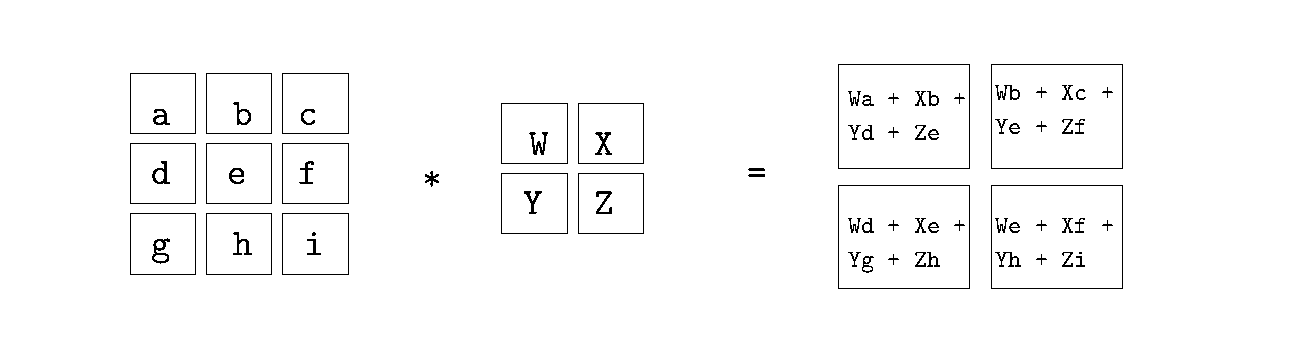
\includegraphics[width=\linewidth]{convolutionexample.pdf}
  \caption{A 2x2 convolution on a 3x3 matrix}
  \label{fig:convolution}
\end{figure}


Using kernels makes convolutional neural networks much more parameter efficient than fully-connected networks as they allow sparse interactions as there is not a parameter connecting each input unit with each output unit. However, as convolutional networks typically work with very high dimensional input, as in images with thousands of pixels, the cost of convolutional neural networks can still be very high overall. \\

Further, latency of convolutional neural networks increases drastically as kernel sizes increase and the number of required mult-adds increases near quadratically. This is the case with standard convolutions where one kernel of a given size produces output for each x coordinate, y coordinate and input channel. Techniques to reduce latency and model size using different convolution techniques is discussed at length in Section 2.2. \\

Typically these convolutional operations are followed by pooling operations which reduce the size of the feature maps. For example, a max pooling operation would just take the largest value in a matrix. Any aggregate function can be used, however, such as an average. This both has the effect of producing condensed, summarised representations of the feature maps, which allows higher-order features to be convolved on in later layers, but also it provides invariance to translation. Intuitively, this is not a feature that is beneficial in hand orientation inference where the location of a feature, such as an edge, is of the utmost importance in determining the orientation. \\

It is also possible to downsample during the convolution phase. This is done by setting a stride greater than 1. So in the previous example where the kernel is applied to every possible combination of units from the input, then if the stride is set to 2 it would 2 pixels across, not 1, when applying the kernel to following set of units. This has the effect of lowering the dimensionality of the following feature map but does not aid in building higher level features as pooling does.\\

It is most typical for a convolutional neural network to be comprised of alternating layers of standard convolutions and pooling operations before the a feature map is flattened and past into several fully-connected layers. The fully-connected layers at the top can easily contain the vast majority of parameters due to the lack of sparse interactions. In a classification or regression task they serve to accurately output a class label or value. Although, in many cases they are not required as is the case with SqueezeNets [8] which achieves state-of-the-art accuracy whilst being fully convolutional. \\

In [27] it is noted that convolutional neural networks have played a significant role in bring deep learning into the forefront of machine learning generally by allowing great advances in accuracy, solving many commercial applications and winning many contests. [27] states that is not completely clear the exact reason that convolutional neural networks were able to achieve such great improvement in accuracy.\\ 

Advances in 2012 when Khrizhevsky won ImageNet by training a deep convolutional neural network on a GPU allowed great improvements in training time which of course allows for more efficient parameter tuning. It would be unreasonable to attribute all of their success to this and other architectural advances have allowed for training of much deeper networks which are generally easier to train without diverging. One example of these architectural advances are residual connections which allow feature maps to skip layers and makes training more robust because... . These were popularies in [....] but are seen as a variation in training in other works, most relevant to this work is in SqueezeNets [27] original experiments.
[p.350 DL]

\subsubsection{SqueezeNets}
SqueezeNets were described briefly in the literature review section. A more detailed description is necessary in order to fully understand the difference between the models that will be used in this work. Typical SqueezeNet architecture is comprised of Fire modules (figure 2) along with convolutional layers at the top and bottom of the network. The original SqueezeNet architecture consists of 8 Fire modules between the top and bottom convolutional layers. The features maps pass through global average pooling after the final convolutional layers before being passed to the output layer.\\

\begin{figure}[!b]
  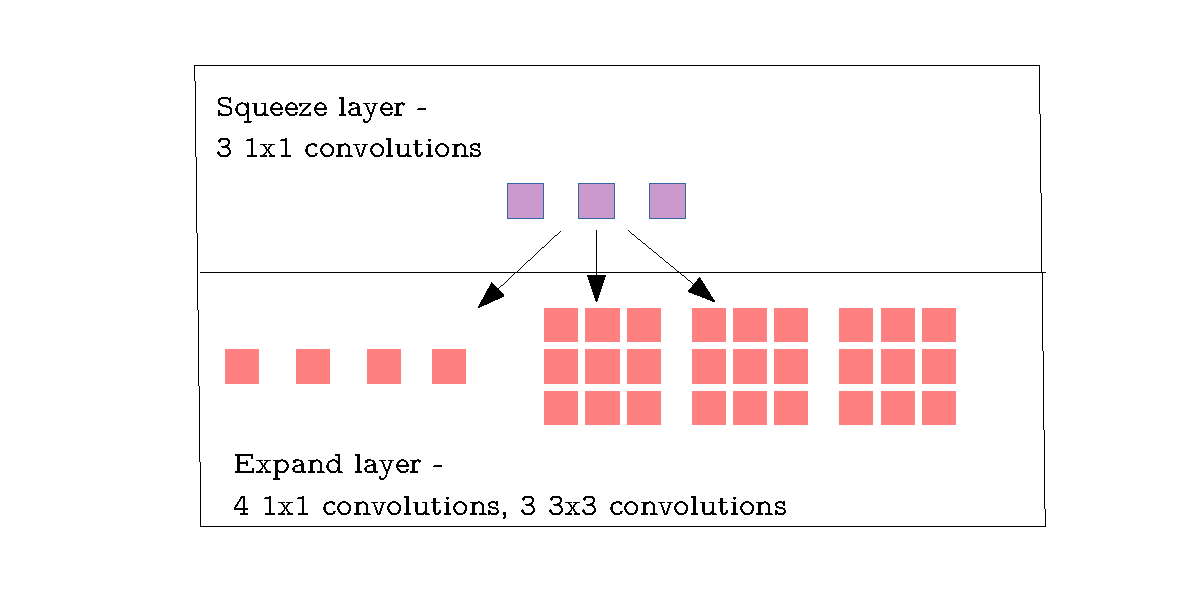
\includegraphics[width=\linewidth]{fire.pdf}
  \caption{A Fire Module}
  \label{fig:dwconvolution}
\end{figure}

***inception towers
Fire modules allow for great parameter efficiency whilst still retaining larger activation maps within a layer. The squeeze layer in a Fire module is comprised of solely 1x1 filters. Typically, there are few filters in the squeeze layer in order to restrict the number of input channels to the expand layer. Of course, as the number of parameters in the expand layer is both dependent on the dimensionality of the filters and the number of input channels, this will reduce the overall cost of any given configuration of filters within an expand layer. Note the 1x1 convolutions in the squeeze layer also have the more generic benefit of having quadratically fewer parameters than filters as the width and height grow. \\

The expand layer consists of 1x1 and 3x3 convolutional filters which can produce more expressive feature maps. With the expand layer the size of feature maps can be relatively large and then in conjunction with the squeeze layers the number of parameters can be reduced quickly at each layer. This benefit is utilised by expanding the output from the squeeze layer in all the layers quite heavily in the early layers and only reducing the amount of expansion, which in effect is the amount of downsampling, until much later in the network which increases accuracy as the output maps remain large for longer.\\

The design of fire modules then provides three hyperparameters. The number of 1x1 filters in the squeeze layer, the number of 1x1 filters in the expand layer and the number of 3x3 filters in the expand layer. How these hyperparameters change throughout the network is controlled by metaparameters. \emph{Freq} is a metaparameter which is the number of layers before the number of expand filters is increased by \emph{incr}. These both scale the /emph{base} metaparameter which set the number of filters in the first expand layer. As the expand filters increases, the number of squeeze filters is controlled by \emph{squeeze ratio} so the number of squeeze filters can increase at the same rate. The percentage of 1x1 filters compared to 3x3 filters within an expand layer is controlled by another metaparameter \emph{pct 3x3}. \\

The original implementation of SqueezeNet has the following metaparameters: base = 128, incr = 128, pct 3x3 = 0.5, freq = 2, and squeeze ratio = 0.125. These were used along with ReLU activations are used between the squeeze and expand layers. 50\% Dropout is used between the final fire module and the final convolutional layer. In [9] experiments on the metaparamets are performing on ImageNet showing that increasing \emph{squeeze ratio} from 0.125 (4.8MB model) to 1 was shown to increases in accuracy from 80.6\% to 86\% with a plateau at 0.8 (19MB model) beyond which only model size increases. Likewise a similar plateau exists for \emph{pct 3x3} where only model size increases.\\

More complex SqueezeNet architectures are also developed in [9] using residual connections which avoid bottlenecks as information can flow directly to later layers. Standard residual connections was shown to increase accuracy the most, from 80.3\% to 82.5\% whereas more complex residual connections which themselves contain 1x1 convolutions only increase accuracy to 82\% whilst increasing model size unlike simple connections.\\

\subsubsection{MobileNets}

MobileNets, like SqueezeNets, are fundamentally different to Vanilla CNNs due to their base convolutional layers which utilise 1x1 convolutions. In MobileNets' case these are depthwise separable convolutional layers. Depthwise separable convolutions are factorized convolutions which separate standard spatial convoltuions into depthwise convolutions followed by 1x1 pointwise convolutions.\\

\begin{figure}[!b]
  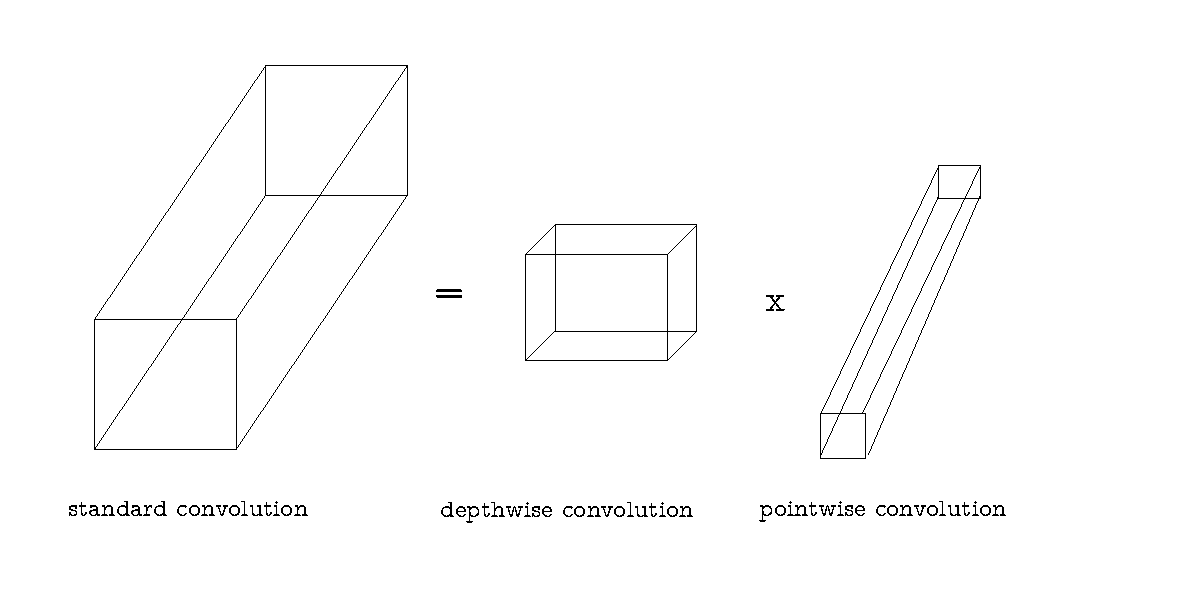
\includegraphics[width=\linewidth]{separableconv.pdf}
  \caption{A standard convolution decomposed into depthwise and pointwise convolutions}
  \label{fig:dwconvolution}
\end{figure}

p. 350 dl
For instance, a 2-dimensional kernel which can be expressed as an outer product of 2 vectors, one in the x direction and one in the y direction, would be a separable kernel. It is equivalent to perform convolutions using these 2 1-dimensional vectors and then combine their outputs using 1x1 pointwise convolutions. This technique scales to multi-dimensions, for instance when there are multiple feature maps deriving from different kernels. The efficiency gains in parameters are quadratic in that if you have \emph{d} dimensions and kernels which are \emph{w} units wide, the cost of convolution operation would be \emph{O($W^d$)} for separable convolution and \emph{O(W * d)} for standard convolutions. [27] \\

A diagrammatic representation of a depthwise separable convolution is shown in figure 3. A standard convolution on the left hand side is applied to every input channel hence its depth. This is equivalent to convolving depthwise first and then multiplying these by 1x1 pointwise convolutions which allow the parameters to be applied to each input channel, or depth. An example depthwise separable convolution layer will contain multiple depthwise and pointwise convolutions and is shown diagrammatically in figure 4.\\

\begin{figure}[h]
  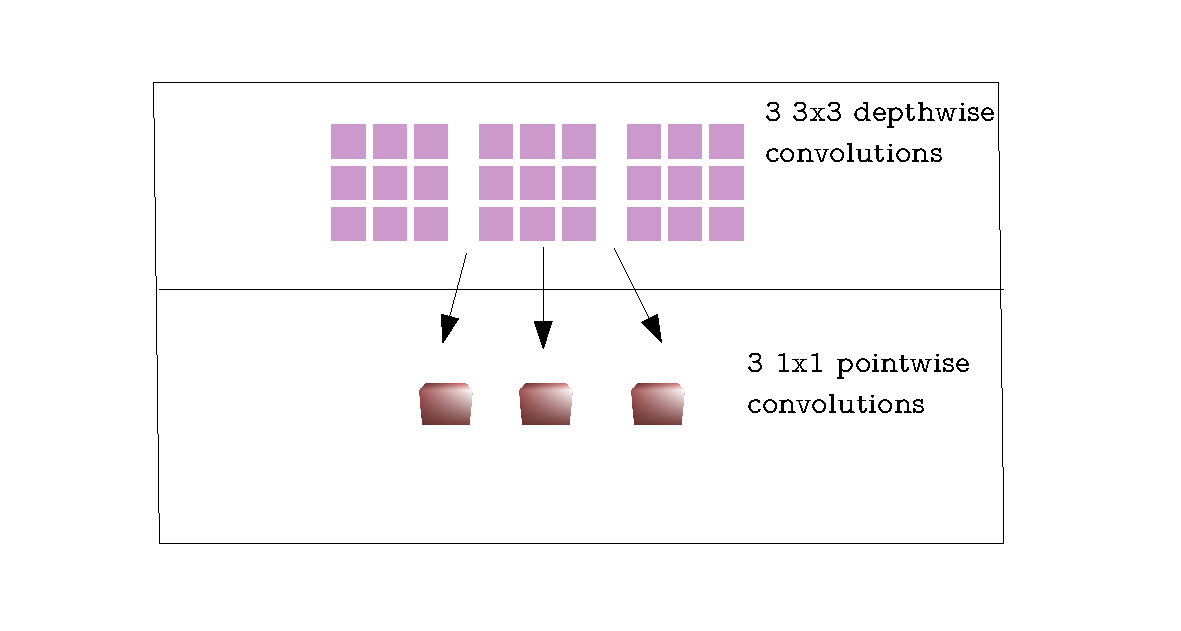
\includegraphics[width=\linewidth]{dwlayer.pdf}
  \caption{A depthwise separable convolutional layer}
  \label{fig:dwconvolutionlayer}
\end{figure}


This has the advantage of having 8-9x fewer parameters as in a standard convolution, the spatial height and width of the filter, the number of input channels, the number of output channels and the feature map sizes all compound multiplicitavely into a very large number of parameters. As in [x] if we let \emph{$D_{F}$} and \emph{$D_{K}$} represent the height or widths of a feature map and kernel height respectively, and further let \emph{M} represent the number of input channels and \emph{N} the number of output channels, then the number of parameters in standard convolution can be expressed as: \[\emph{$D_{F}$} \cdot \emph{$D_{F}$} \cdot M x N \cdot \emph{$D_{K}$} \cdot \emph{$D_{K}$} + M x \cdot N x \] Whereas if the convolution is separated into its depthwise and pointwise components then the cost is: \[\emph{$D_{F}$} \cdot \emph{$D_{F}$} \cdot M \cdot \emph{$D_{K}$} \cdot \emph{$D_{F}$} \cdot \emph{$D_{F}$} \cdot \emph{$D_{F}$}\]\\

It is important to note at this point that it is not of major use to purely put emphasis on number of parameters when measuring the efficiency of a model. This is because number of mult-adds does not necessarily scale uniformly with latency. On a per-module basis, that is number of parameters in a Fire module for example, number of parameters would of course scale fairly uniformly with latency. However, over an entire model for example, the number of mult-adds can be reduced using pruning. This creates a sparse model with bottlenecks and the latency of the model will not reduce at the same rate as number of mult-adds. [1] \\

to add: The base structure for a MobileNet is a layer of full convolutions followed by depthwise separable convolutions all with ReLU activation functions. Batch normalisation and strided convolution downsampling is performed between each layer. Average pooling is then performed before output is passed to the fully-connected layers.\\


\subsection{Network Architecture and Training}
A multi-input architecture will be used, as is typical for many other works related to hand-orientation and hand-pose estimation. Specifically, a three input network where one network will take image sizes of 128x128, 64x64 and 32x32. The resultant feature maps of each network will be flattened and concatenated before being passed to fully-connected layers which sit on top of these networks. This structure is shown in figure 5.\\

\begin{figure}[h]
  \centering
  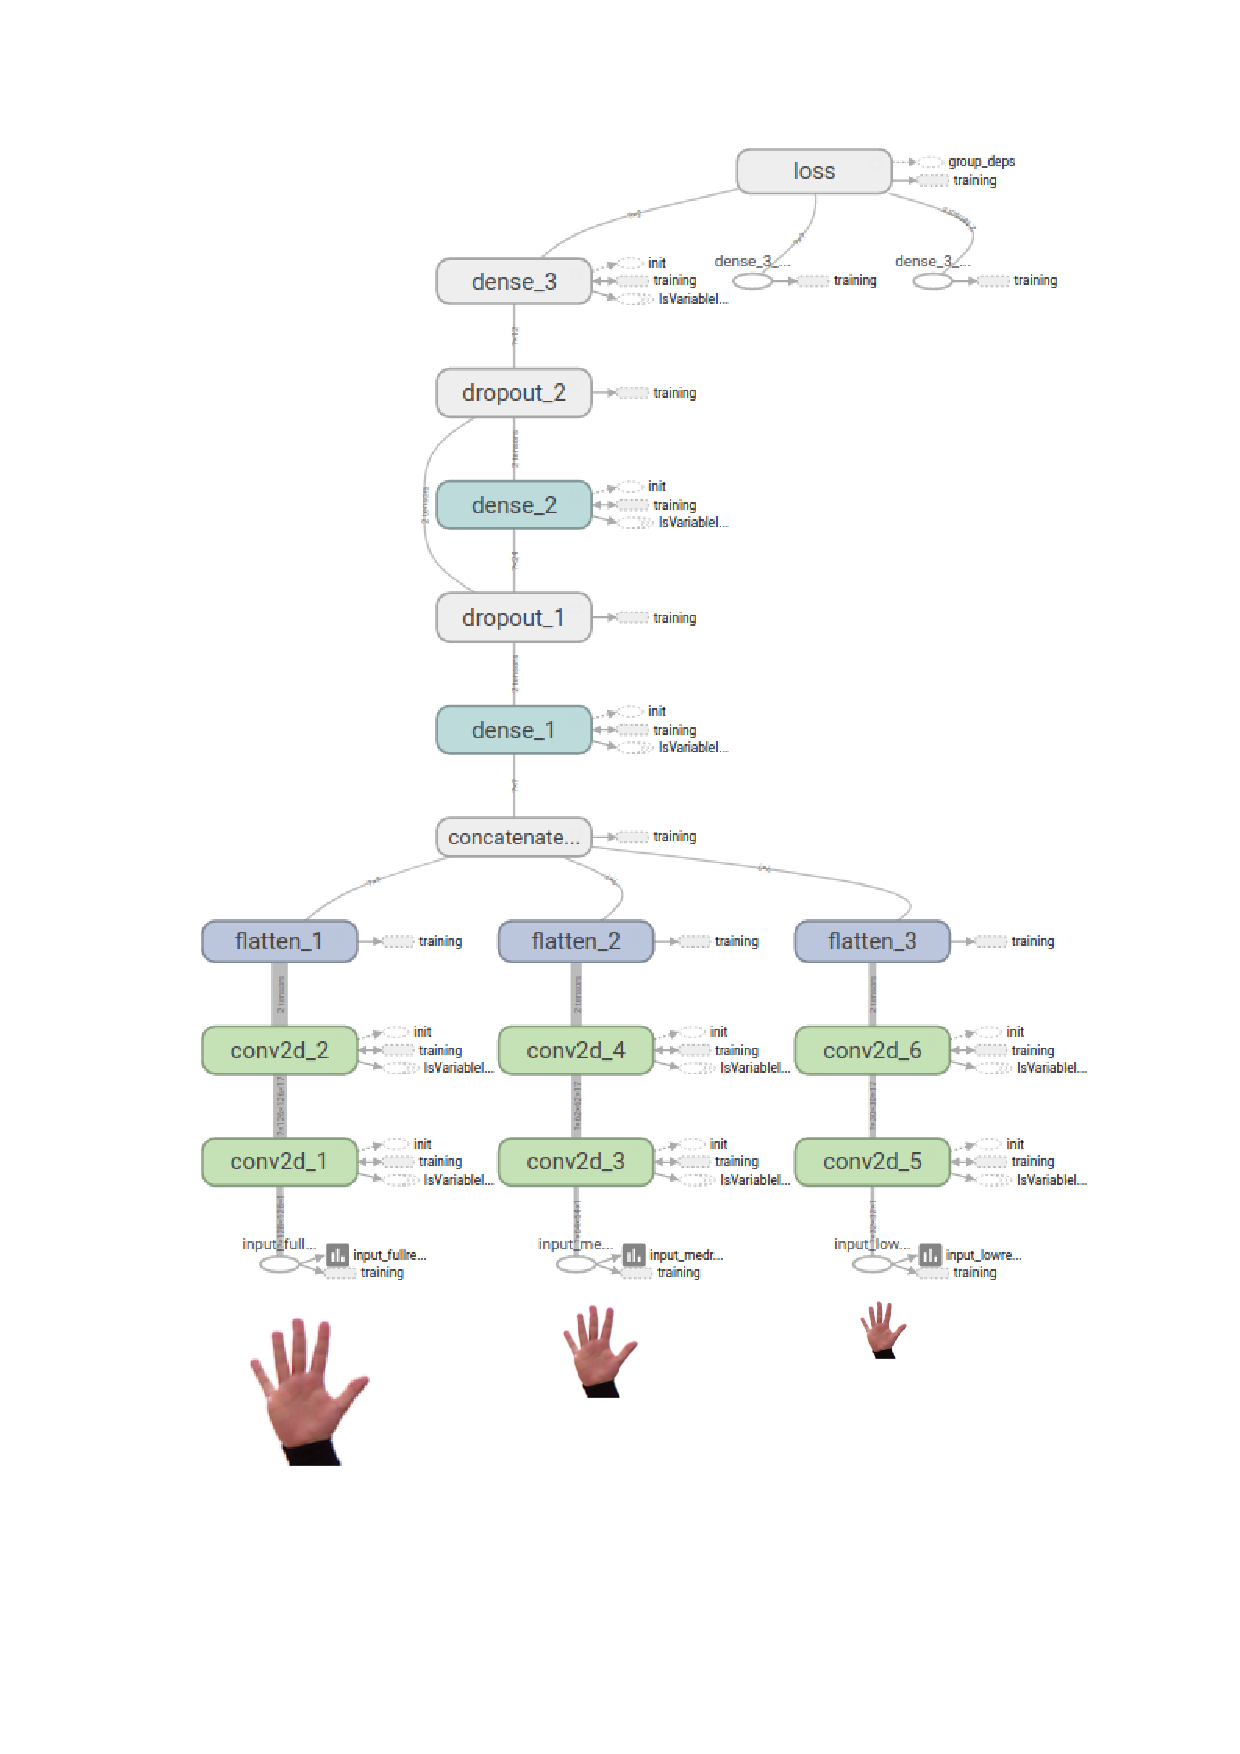
\includegraphics[scale=0.4]{tbgraph.pdf}
  \vspace*{-15mm}
  \caption{Multiresolution network architecture}
  \label{fig:multiinput}
\end{figure}

To avoid saturation of gradients in the network, rectified activation units will be used. Standard rectified linear units (ReLU hereafter) reassign all negative values to zero and lets positive values pass unchanged. This makes ReLUs computationally very efficient compared to parametric non-linear activation functions such as a sigmoidal. However, as all negative values are set to 0, large updates can cause gradient not to be able to pass through the ReLU.\\

This problem can cause large parts of the network to die and results in relatively sparse network. This sparsity was often attributed to the state-of-the-art performances of ReLU. However, advances in rectified activation unit design brought forward units which allow negative gradients to pass. An example is LeakyReLU which scales negative values with a large denominator however this denominator can be parametrised to let more gradient through. Randomized leaky rectified units (RRelu) randomize the amount of negative gradient that passes through and in [6] outperformed other rectified activation units due to the additional regularization.\\

[6] also points out that LeakyReLU units which were very leaky, as in they let more gradient through, outperformed less leaky ones which are more common. It is important to note, however, that the difference in performance between different rectified activation units in [6] is very marginal.\\

Also, using a fairly complex network structure on an intricate task with a fairly small dataset, particular attention must be paid to the initialization strategy of the network weights. The efficacy of weight intialization and its ability to allow convergence of deep networks was brough to the forefront in [22] with Xavier intialization. For ReLUs, however, the optimal weight strategy of giving weights variance of $1/N$ (where N is the number of units in a layer) was shown not to hold true. Specifically, in [24] it is shown that the optimal variance weights in ReLU based networks is in fact $2/N$ and in many cases networks fail to converge under Xavier intialization. This is not merely empirically observed but the result is rigorously proved in [23].\\

Add dropout

\subsection{Training Configuration}
\subsubsection{Dataset}
The dataset used is the same which is collected by Asad in [17]. The dataset consists of 9717**** RGB images of 13 different participants hands against a plain background. Ground truth orientation is inferred by simultaneously capturing depth images of the participants' hands using a Kinect sensor. The plane that implicitly sits across the 3D point cloud is calculated using the RANSAC algorithm on these coordinates. From this plane equation the normal vector can be calculated as the transpose of the x, y and z components of the plane equation. These inverse cosine of these x and y components are used to calculate the azimuth and elevation angles which provide the ground truth labels for training. Formally, as shown in [1], this is:

\[\emph{$n_{0}$} =  \emph{$xn_{x}$} + \emph{$yn_{y}$} + \emph{$zn_{z}$}\]

\[\emph{$N$} =  [\emph{$n_{x}$},\, \emph{$n_{y}$},\, \emph{$zn_{z}$}]^T\]

\[\emph{$\Phi_{k}$} =  \emph{$cos^{-1}n_{x}$}\]

\[\emph{$\Psi_{k}$} =  \emph{$cos^{-1}n_{y}$}\]

RANSAC is well suited to this task as it takes a random sample of points in each iteration making it more resilient to outliers. Outliers in this case could be of particularly large effect as the hand takes up a fairly small proportion of the image. This means small errors can be amplified into larger ones causing inaccuracies in the labels and creating difficulties in the training process where very similar images have vastly different labels.[17]\\

In [17] a painting game was also developed during the data collection process, where a user is given feedback showing how much of the orientation space they have managed to fill with sufficient samples. This was in response to earlier datasets which had inconsistencies and gaps in orientation space as users failed to provide sufficient examples for the entirety of orientation space. This then provides a consistent and balanced dataset already from the collection phase and does not require and post-processing to balance the dataset.

\subsubsection{Error Metric}
The networks are configured to output both the elevation and azimuth angle. This obviously has the benefit of these error signals being able to propagate back through the network separately. As in [17] we analyse the error of each of these angles separately in order to understand the performance of the models. It was typical in [1]'s experiments that certain examples would perform well in one angle but be unable to gain accuracy in the other angle.\\

In order to compare results with [17], both error metrics are adopted. Mean average error (of azimuth and elevation angles) and combined mean average error (MAE and CMAE hereafter).

Add figure of azimuth and elevation. + taking mean implicit

\subsubsection{Software Configuration}
All models were built using Keras, which is a high level API for constructing neural networks. It uses other frameworks for backends. For this work TensorFlow was selected as this is support on Google Cloud ML Engine. \\

Standard convolutional layers and fully-connected, or dense, layers are obviously supported in the base library. The components which make up SqueezeNets and MobileNets are not part of the base library and had to be implemented separately. \\ 

MobileNets in their original implementation are available to import as  a model in Keras, but this provides no flexibility in altering structure and would not support a multiresolution architecture. To achieve this, an adaption of the base separable convolution class in Keras can be used to construct a depthwise separable convolutional layer [Malli]. This layer can then be used to build custom depthwise convolutional blocks which can be used modularly as if they were standard layers and there is no strict confinement to the base MobileNet structure. \\

A similar approach was taken to implement SqueezeNets. The base building blocks, in this case Fire modules, were implemented separately allowing complete control over the structure of the network. Using [Malli] as a base for the modules, I modified them to adapt to all of the hyperparameters mentioned in the original paper [], and modified the model construction to both be suitable for regression and multiresolution architectures. \\

Testing was done by ensuring pixel values and label values were within a strict range at all parts of the pipeline. Network configuration was tested visually using TensorBoard. This shows the exact shape of the graph along with histograms of the weights during training. This  allows confirmation that the network architecture is correct in addition to whether any of the modules are behaving problematically, as the distribution of the weights may be abnormal.

\subsubsection{Training Pipeline Configuration}
To streamline the training pipeline all image resizing and grayscaling was performed locally beforehand and the various resolutions were then kept on cloud storage so the correct image formats could be served directly to the models during training. This had to be performed in batches to avoid generating a graph of over TensorFlow's 2GB limit, as the resizing was done using TensorFlow's preprocessing module. \\

This leaves only an input generator, which simultaneously performs samplewise standard deviation normalisation, along with the actual training of the model in the pipeline.
The input generator is vital for memory management, as without controlling the input generator's batch size to be sufficiently small, the GPU can run out of memory and the training process is killed. In fact, the entire training process was extremely sensitive and it was necessary to decrease what was a stable batch size just to accomodate slightly larger models or models which did not use pooling. \\

The training pipeline was configured in such a way that ranges of hyperparameters are provided automatically by a hyperparameter configuration file where the ranges are specified. Then multiple parallel trials could take place on cloud. Results of these parallel trials are used in the Bayesian hyperparameter optimisation to choose which value within the range to explore most over a maximum number of trials that is specified. \\

The same hyperparameter optimisation strategy was used for a variety of structural experiments. That is the hyperparameters and structure were not optimized simultaneously but rather in multiple parallel trials. Some structures provided extremely poor, even divergent, solutions and it was much easier to understand what structural characteristics were causing this by separating structure optimization from hyperparameter optimization.\\

A particular good example of this is that due to the small batch size required to manage memory, regularization techniques such as layer-wise batch normalization were very unstable as the normalization was being performed on feature maps of very few samples (8 or fewer). In fact, some hyperparameters showed extreme variance in test error, showing errors between 5 degrees to 50 degrees just by randomizing the order in wich the images were passed into the model. \\

By removing layer-wise batch normalization the model showed strong stability and low test error variance over a variety of hyperparameters and is discussed more in depth in results.  But it is still worth highlighting how the training pipeline configuration influenced the structure of the model. \\


\subsubsection{Optimization Strategy}

Hyperparameter tuning will be performed using Google Cloud ML Engine's implementation of Bayesian optimization on a fixed range of parameters. Bayesian optimization is an alternative to a naive grid search which allows a more efficient exploration of hyper parameter space. Naive grid search wastes a great amount of computation on calculating performance in area of parameter space which is unlikely to yield optimal results.\\

Bayesian optimization works by modelling the function we are interested in optimizing not only using local gradient information but also all past evaluations of the function. In this way, the Bayesian framework makes a probabilistic evaluation of the function during training and chooses hyperparameters than have the highest probability of improving the model's performance.\\

 There are drawbacks to Bayesian optimization in that the covariance functions which controls the distribution of functions that are evaluated itself has to parametrised and there is little to no theoretical grounding in how to do this. Nevertheless, in [28] in which the framework is proposed state-of-the-art was surpassed by 3\% with significantly less training time than previous approaches. As the training process in this work will be costly, Bayesian optimization will allow a larger hyperparemter space to be explored and is configured in Google Cloud ML to still be able to take advantage of parallel computing which is cited in [28] as a consideration on whether the technique is able to gain significant efficiencies as compared to naive grid search. \\
 
 With such measures being taken to efficiently explore hyperparameter space, it is an an obvious choice to use a standard train-validation-test split will be used to measure performance. K-fold cross validation was deemed too costly.\\




\subsection{Evaluation}

\subsubsection{Evaluation Technique}
The methodology used in this work was to choose a suitable range for a number of hyperparameters that were applicable to each model. For instance, SqueezeNets have several hyperparameters that do not apply to standard CNNs, so it is not possible to have a consistent set of hyperparameters that are optimized over all  models. \\

Each unique set of hyperparameter ranges is then applied separately to several different structures for each model. For example, for the vanilla CNN suitable ranges for kernel size, number of filters, number of neurons in the fully-connected layers and dropout were chosen. This hyperparameter set was then used to calculate performance for structural choices such as how many layers were used in the convolutional parts of the network or whether to include pooling layers. \\

A maximum number of trials was set at 32 for each structural choice and then the Bayesian hyperparameter optimisation framework would select the appropriate hyperparameters to calculate performance for in order to optimise accuracy. \\

As cross-validation is not used, but rather a simple train-test split, in order to estimate generalization error the average error for the top 16 performing network hyperparameter configurations is used to define the accuracy for a given structure. This of course has the advantage of seeing how stable a model is over hyperparameter space at the loss of seeing how stable a model is on being trained on different subsets of the data.\\

Although the dataset was fairly small, it is completely justified not to increase training cost by 5-10x (assuming 5-10 folds). In the end, this would only confirm that one particular set of hyperparameters is likely to generalise the best. Stability of performance in hyperparameter space will allow us to draw similar conclusions.\\

\begin{table}[h!]
  \begin{center}
    \caption{Hyperparameter Ranges}
    \label{tab:table1}
    \begin{tabular}{l|l|l|l}
      \textbf{Hyperparameter} & \textbf{Vanilla} &                          \textbf{SqueezeNet} & \textbf{MobileNet}\\
      \hline
      Kernel size & 2 - 7 & 2 - 7 & 2 - 7\\
      Filters & 5 - 25 & 5 - 25 & 5 - 25\\
      Dropout & 0 - 0.7 & 0 - 0.7 & 0 - 0.7\\
      Fully-connected neurons & 16 - 256 & 16 - 256 & 16 - 256\\
      Bottleneck 1x1s & - & 16 - 256 & - \\
      Squeeze ratio & - & 0.1 - 0.7 & - \\
      Percentage 3x3 & - & 0.15 - 0.75 & - \\
    \end{tabular}
  \end{center}
\end{table}

Structural changes were not as strictly defined and developed during the experimental process. However, they largely revolved around differing the number of convolutional layers, pooling layers, and fully-connected layers. The overall multiresolution structure, including the resolution of the images, was not changed during the process. \\

Latency will also be taken into consideration which will be measured by how many seconds are taken to generate predictions on a given number of images from the original dataset. This will be measured using an i5 CPU which acts as a completely sufficient proxy CPU for one which would be present in a modern mobile phone. Latency will be measured just on the best performing models, in terms of accuracy, and primarily serve as a tool to potentially dismiss the best performing model in favour of a smaller one with similar accuracy. \\

As all models trained in this work will be relatively small, a complete study of latency to accuracy will not be undertaken.. The architectures tested also do not vary significantly in number of layers and so latency is largely driven by kernel size for which there is no strict trade off between latency and accuracy. Also, to serve predictions in real time there must be real time preprocessing involving producing differing resolution images for input and converting these to grayscale, which itself is costly. In this way, model latency is only one factor in overall latency for serving predictions. \\

\subsubsection{Definition of Hyperparameters}
Kernel size represents the width and height of the convolutional filters used. For the standard CNN this size filter is used for each layer. For MobileNets and SqueezeNets this filter size is only applied to the standard convolutional layers. So all Fire modules and depthwise separable convolutional blocks remain comprised of 3x3 and 1x1 convolutions. \\

The filters hyperparameter is simply the number of filters trained in any layer of any model. There were no restrictions as there were for the kernel size. \\

Dropout is the proportion of neurons in the fully-connected layers which are excluded for each example during both the forward pass and backward pass. This is a standard regularization technique and is applied to both layers. \\ 

Fully-connected neurons is the number of neurons in the first fully-connected layer. In each model, the second layer always contained half the amount of the first layer. \\

Bottleneck 1x1s represents the number of 1x1 convolutional filters that the final feature map from a SqueezeNet passes through before the fully-connected layers. Passing through fewer filters will cause the feature maps to become more condensed. \\

Squeeze ratio and percentage 3x3 are described in more detail in Section 3.1.2 and just effect the number of 3x3 and 1x1 filters within a Fire module.

\section{Results}

\subsection{Main Results}
\begin{table}[h!]
  \begin{center}
    \caption{Results}
    \label{tab:table1}
    \begin{tabular}{l|l|l|l}
      \textbf{} & \textbf{Vanilla} &                          \textbf{SqueezeNet} & \textbf{MobileNet}\\
      \hline
      Elevation Angle Error & 10.56$^{\circ}$ & 13.94$^{\circ}$ & -\\
      Zenith Angle Error & 10.52$^{\circ}$  & 9.78$^{\circ}$ & -\\

    \end{tabular}
  \end{center}
\end{table}

Performance was inferior to results gained in [17]. However, the efficient models were able to achieve similar performance to the standard CNN. The better performing efficient models also tended to be larger structurally. For example, the best performing SqueezeNets would typically have 4 Fire modules for each resolution compared to the Vanilla networks 2 convolutional layers.\\

The best performing SqueezeNet had a kernel size of 6, and with fairly high squeeze ratio and pct 3x3 of 0.47 and 0.723 respectively. The only characteristic it shared with the best performing Vanilla architecture is that it required heavy regularization with Dropout of 0.5.\\

However, it is not indicative of this particular training process overall to focus on specific configurations as many similarly configured models would become constant predictors during training. In fact, differing ways of processing the data or configuring the network led significantly worse results than the general frameworks which allowed the acceptable results as shown above. For example, mean standard deviation normalisation of the pixel values caused significant drops in performance and the reasons for which are unclear as all normalisation was performed on a global basis, not batchwise, in order to stabilise the process. \\

The stochastic optimization process in ADAM, was insufficient in itself to prevent many configurations getting stuck early on in training, in terms of accuracy. This was even in conjunction with using very leaky ReLUs to avoid negative input being culled early in the network and to allow as much loss information to flow through the network during training.
It was troublesome for the Bayesian optimization process that many configurations got stuck or became constant predictors as it is harder to build a distribution of how hyperparameters and accuracy interact. Poorer models tended to become constant predictors and in this way their is little information to differentiate between them . \\

Attempts to increase accuracy by using more global features maps failed. This was done by utilising pooling operations. It is possible that using lower resolution images instead of pooling could have increased accuracy but this is of course largely speculation. \\


\subsection{In Depth Analysis of Training Process}
It was often the case that models with similar parameters would show wildly different properties in terms of loss. This is demonstrated in this section by looking at the training of two Vanilla CNNs. One showed strong convergent properties and the other divergent properties as shown in figure \ref{fig:loss}. These models had parameters ............. and identical structure and data preprocessing. The poor model's loss never approaches the good model's loss first epoch loss even.\\

Looking at the histogram distribution of kernel and bias parameters in conv2d\_1 which is the first full resolution layer as seen in figure \ref{fig:multiinput}. The good model's parameters in figure \ref{fig:goodearlyweights} are in fact fairly similar to those in the bad model as shown in \ref{fig:badearlyout} as they are both fairly evenly distributed around 0. \\

However, when looking at the outputs from these layers as shown for the good model in figure \ref{fig:goodearlyout} and the poor model in figure \ref{fig:badearlyout} there is a clear difference. The poor model's outputs get stuck below 0 whereas the good model's outputs remain distributed around 0. My choice of activation function being LeakyReLU in part was to prevent situations like this, and in fact the LeakyReLUs were parametrised to be especially leaky with $\alpha$ being 0.1, meaning negative values are not culled completely and allowed to flow. This is also true of the selection of ADAM as an adapative learning rate to help the model escape such traps during training.\\

Although literature suggests the He initialisation is more theoretically sound for ReLUs, Xavier intialisation was strictly better performing for this better task. Although, the results would suggest otherwise, my initialisation strategy may be in part to blame for these divergent properties. It is difficult to do much more than speculate however given that Xavier outperformed He overall in this task. \\

These primarily negative outputs were shown in most other convolutional layers for the poor performing model. Looking at the implications this has for the dense, fully-connected layers later on in the network it is possible to gain further insight into the training process. These are showing in figures \ref{fig:gooddenseout} and \ref{fig:baddenseout} for the good and poor model respectively. \\

There is a clear divergent, negative drift of the dense units' biases, showing there is no major corrective event during the training process. In addition to this, looking at the output from the dense layer for poor model in figure \ref{fig:baddenseout} as compared to the good model, the poor model again shows an extremely negatively scewed distribution compared to the good model. There is also a shock event in the 7th epoch as the weights collapse to extremely negative value.\\

It is difficult to pinpoint the exact reason for this and why other models were resilient to this shock event. It is possibily an over reaction as other filters are unable to pick up on features and there was perhaps some conversion artefacts that caused this, but this is merely speculation. \\

Add what we learn from this and how this is likely cause, and tblogs were not gathered for other models during training

\subsection{Analysis of Successful and Unsuccessful Examples}
\begin{table}[h!]
  \begin{center}
    \caption{Successful Vanilla CNN error breakdown}
    \label{tab:tablebreakdown}
    \begin{tabular}{l|l|l|l|l}
      \textbf{} & \textbf{Mean $\zeta$} &  \textbf{Std $\zeta$} & \textbf{Mean $\epsilon$} &  \textbf{Std $\epsilon$}  \\
      \hline
      Successful Azimuth Set & 19.76$^{\circ}$ & 11.64$^{\circ}$& 13.27$^{\circ}$ & 11.03$^{\circ}$ \\
      Successful Elevation Set & 18.18$^{\circ}$  & 15.78$^{\circ}$ & 12.92$^{\circ}$ & 8.12$^{\circ}$\\
      Unsuccessful Azimuth Set & 17.51$^{\circ}$ & 9.75$^{\circ}$ & 19.38$^{\circ}$ & 9.76$^{\circ}$\\
      Unsuccessful Elevation Set & 19.51$^{\circ}$  & 10.51$^{\circ}$& 25.15$^{\circ}$ & 9.87$^{\circ}$\\
    \end{tabular}
  \end{center}
\end{table}

\begin{table}[h!]
  \begin{center}
    \caption{Successful MobileNet error breakdown}
    \label{tab:tablebreakdown}
    \begin{tabular}{l|l|l|l|l}
      \textbf{} & \textbf{Mean $\zeta$} &  \textbf{Std $\zeta$} & \textbf{Mean $\epsilon$} &  \textbf{Std $\epsilon$}  \\
      \hline
      Successful Azimuth Set & 16.34$^{\circ}$ & 11.29$^{\circ}$& 17.59$^{\circ}$ & 9.04$^{\circ}$ \\
      Successful Elevation Set & 19.27$^{\circ}$  & 12.44$^{\circ}$ & 19.34$^{\circ}$ & 12.14$^{\circ}$\\
      Unsuccessful Azimuth Set & 14.75$^{\circ}$ & 11.82$^{\circ}$ & 13.28$^{\circ}$ & 10.73$^{\circ}$\\
      Unsuccessful Elevation Set & 14.74$^{\circ}$  & 11.58$^{\circ}$& 20.07$^{\circ}$ & 11.10$^{\circ}$\\
    \end{tabular}
  \end{center}
\end{table}

\begin{table}[h!]
  \begin{center}
    \caption{Successful SqueezeNet error breakdown}
    \label{tab:tablebreakdown}
    \begin{tabular}{l|l|l|l|l}
      \textbf{} & \textbf{Mean $\zeta$} &  \textbf{Std $\zeta$} & \textbf{Mean $\epsilon$} &  \textbf{Std $\epsilon$}  \\
      \hline
      Successful Azimuth Set & 15.86$^{\circ}$ & 12.33$^{\circ}$& 14.60$^{\circ}$ & 8.39$^{\circ}$ \\
      Successful Elevation Set & 19.01$^{\circ}$  & 10.75$^{\circ}$ & 14.76$^{\circ}$ & 11.14$^{\circ}$\\
      Unsuccessful Azimuth Set & 18.00$^{\circ}$ & 10.90$^{\circ}$ & 22.18$^{\circ}$ & 10.06$^{\circ}$\\
      Unsuccessful Elevation Set & 20.20$^{\circ}$  & 12.13$^{\circ}$& 18.99$^{\circ}$ & 11.43$^{\circ}$\\
    \end{tabular}
  \end{center}
\end{table}

\begin{figure}[h]
 \hspace*{0cm}
  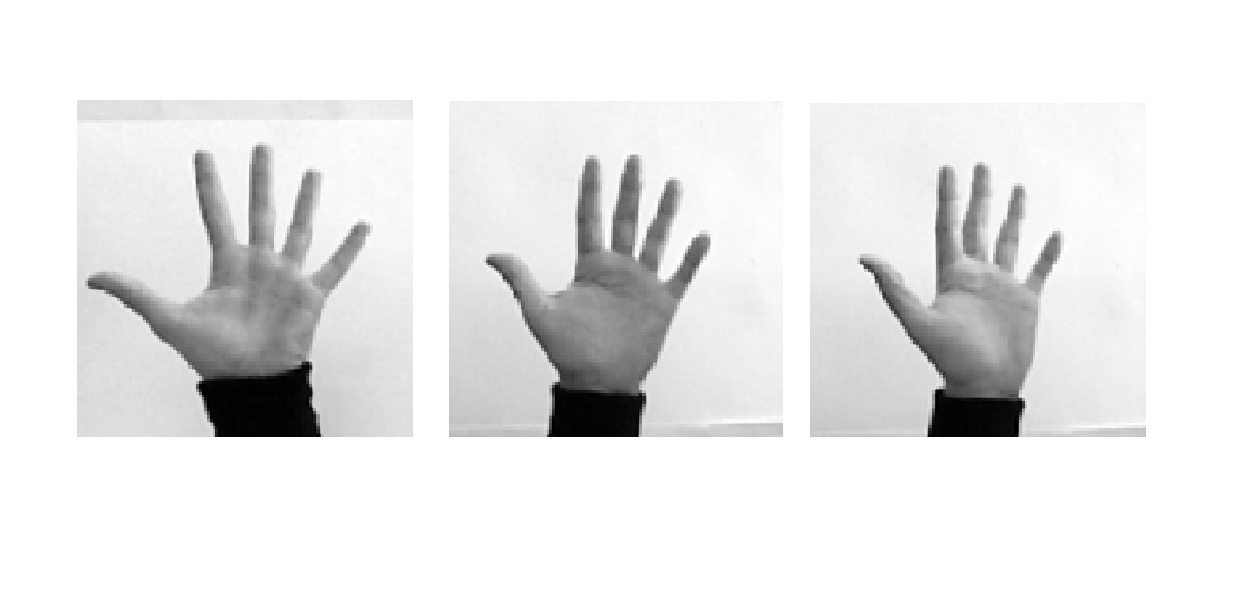
\includegraphics[scale=0.6]{goodz.pdf}
   \vspace*{-21mm}
  \caption{Examples succesfully predicted by model}
  \label{fig:goodz}

\hspace*{0cm}
  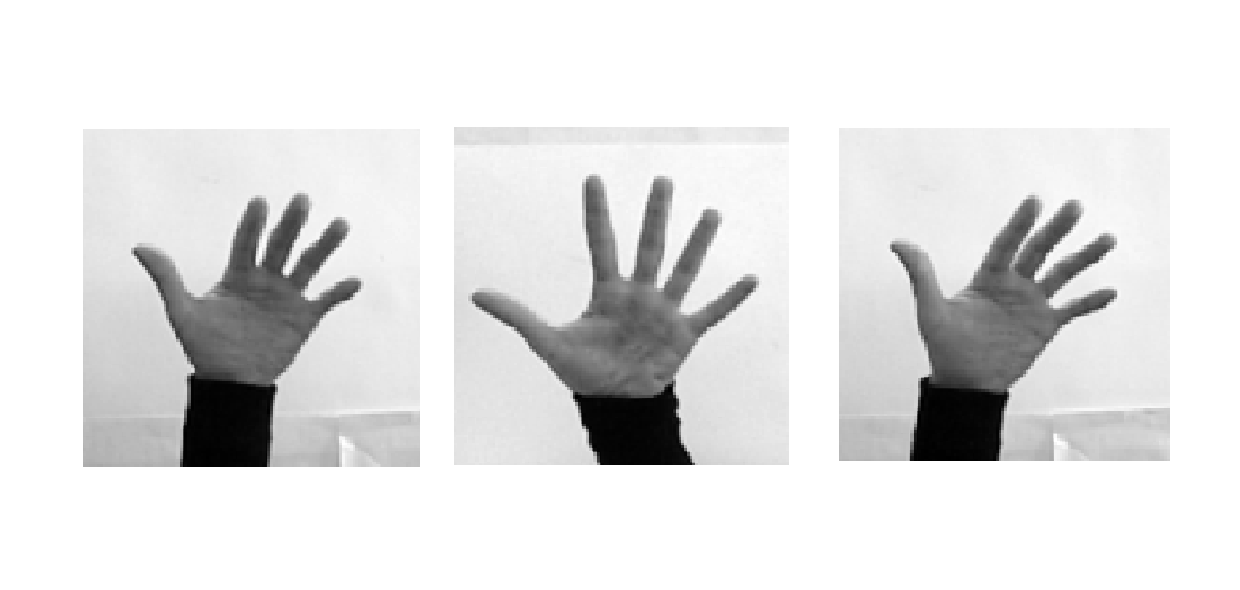
\includegraphics[scale=0.6]{badz.pdf}
  \vspace*{-18mm}
  \caption{Examples unsuccesfully predicted by model}
  \label{fig:badz}

\end{figure}



In this section, I do not analyse the results of the unsuccessful models as detailed in section 5.2 as these models resulted in a constant predictor and so analysing any distribution of angles related to the errors is meaningless as it would only reflect the distribution of the dataset in relation to the constant value. However, I do split the examples into those which were classified successfully, that is below 5 $^{\circ}$, and unsuccessful, that is above 15$^{\circ}$. \\

Looking at table \ref{tab:tablebreakdown} there are several expected, and generic, observations worth highlighting. First, the mean absolute zenith angle is generally larger for the unsuccesfully predicted examples. The std of these angles is similar to those of the successful examples showing again the set generally shows larger azimuth angles. 
This is unsurprisingly shown to a stronger degree by those in the unsuccessful azimuth set. \\

Looking at examples in figure \ref{fig:badz} it becomes obvious why such examples are challenging to predict without depth information. These are those where there is little azimuth rotation to leaving less information for the model to infer about elevation except distortion of the general hand shape. \\


\subsection{Speed Checks}
In this section I do not perform a general comparison of latency against performance. These general comparisons are available in SqueezeNets' [] and MobileNets' [] original papers. Further to this, my training results were very unstable as shown in 5.2 and so would not give a meaningful comparison of latency and performance, as I am not giving up latency for performance as some larger models performed significantly worse than smaller models. \\

This section rather aims to show the suitability of the best performing models for real-time application. In this way, this section aims to confirm my generic preference for smaller models during the training process and whether it has resulted in fast enough models, capable of serving predictions at a smooth frame rate (30 FPS).\\

\begin{table}[h!]
  \begin{center}
    \caption{Performance of Best Performing Models}
    \label{tab:speed}
    \begin{tabular}{l|l|l|l}
      \textbf{} & \textbf{Vanilla CNN} &  \textbf{SqueezeNet} & \textbf{MobileNet}  \\
      \hline
      Examples predicted per second & 56.8 & 54.3 & 41.6 \\
      Model Size & 96.9 MB  & 0.45 MB & 0.28 MB \\
      Number of Parameters & 8,070,794 & 13,559 & 9,155\\
    \end{tabular}
  \end{center}
\end{table}

Table \ref{tab:speed} shows that all the models are more than capable of serving predictions in real-time. However, due to the models being multiresolution the prediction serving has other processes besides producing output from the three different resolution images. The raw input from the camera first has to be resized to the three resolutions, converted to grayscale and the pixel values to be scaled between 0 and 1 which is a significant process in itself.


\section{Discussion}
All three architectures were implemented successfully and gained accurate results with models capable of serving predictions in real-time. In this sense, the project was a success but given the fact that the results were inferior to those in [17] it allows reflection on what else would have been valuable to do and where performance gains could be gained. \\

There are several other benchmarks that I believe would be worthwhile in comparing the aptitude of these architectures. For example, using images with depth information instead of purely RGB would possible allow these architectures to perform much better compared to the ML-RF technique. This is because still only the CNNs would be able to utilise the non-contour pixels, which now would contain more meaningful depth information compared to just skin colour. This would be a reasonable comparison to make as depth perception is becoming increasing commonly in modern handheld devices. \\

Before undertaking modelling on depth information, it would be of worth to understand whether the multiresolution aspect of these architectures provides a significant, if any, increase in discriminatory power. This would be of value both for RGB and depth images. This would be a trivial additional experiment to gain results using a single resolution architecture, and in hindsight a valuable one for this particular work where all the models achieved such similar performance. Although results in literature clearly show a preference for multi-input networks, this was for hand pose estimation and it is still unclear whether the decreased training capacity of a single resolution network could be beneficial for this particular task. \\

I also would now value having more variation in input. I could have taken better advantage of the multi-input capabilities of the networks and used the contour features as in [17] instead of the medium resolution images. This would have provided further evidence of any benefits of the multi-input architecture which could guide following work. \\

Given the fact that so many models failed to converge, I am hopeful that better results could have been gained if a more extensive hyperparameter optimization strategy could have been implemented. The possibility of implementing this was largely impeded  by memory management which was troublesome during the training process. Batch size had to be set to one for certain configuration to even compile. In addition to this, as garbage collection is not instantaneous, those configurations which did compile would often fail later on in training whilst storing intermediate results. This forced me to set batch size to 1 for all experiments in order to ensure the job would finish. This did not allow full utilisation of the parallel processing capabilities of GPU and lengthened training time with some epochs for larger configurations lasting over one hour. It was then unfeasibly costly to perform significantly more extensive hyperparameter optimization. \\



\section*{References}
\begin{enumerate}
\item Howard, A. G., Zhu, M., Chen, B., Kalenichenko, D., Wang, W., Weyand, T., ... \& Adam, H. (2017). MobileNets: Efficient convolutional neural networks for mobile vision applications. \emph{arXiv preprint arXiv:1704.04861}.
\item Chollet, F. (2016). Xception: Deep Learning with Depthwise Separable Convolutions. \emph{arXiv preprint arXiv:1610.02357}.
Chicago	
\item Tompson, J., Stein, M., Lecun, Y. \& Perlin, K., 2014. Real-time continuous pose recovery of human hands using convolutional networks. \emph{ACM Transactions on Graphics (ToG)},33(5), p.169.
\item Oseledets, I. V. (2011). Tensor-train decomposition. \emph{SIAM Journal on Scientific Computing}, 33(5), 2295-2317.
Chicago	
\item Novikov, A., Podoprikhin, D., Osokin, A., \& Vetrov, D. P. (2015). Tensorizing neural networks. \emph{Advances in Neural Information Processing Systems} (pp. 442-450).
\item Xu, B., Wang, N., Chen, T., \& Li, M. (2015). Empirical evaluation of rectified activations in convolutional network. \emph{arXiv preprint arXiv:1505.00853}.
\item Chen, W., Wilson, J., Tyree, S., Weinberger, K., \& Chen, Y. (2015, June). Compressing neural networks with the hashing trick. \emph{International Conference on Machine Learning} (pp. 2285-2294).
\item Iandola, F. N., Han, S., Moskewicz, M. W., Ashraf, K., Dally, W. J., \& Keutzer, K. (2016). SqueezeNet: AlexNet-level accuracy with 50x fewer parameters and< 0.5 MB model size. \emph{arXiv preprint arXiv:1602.07360}.
\item He, K., \& Sun, J. (2015). Convolutional neural networks at constrained time cost. \emph{Proceedings of the IEEE Conference on Computer Vision and Pattern Recognition} (pp. 5353-5360).
\item Szegedy, C., Vanhoucke, V., Ioffe, S., Shlens, J., \& Wojna, Z. (2016). Rethinking the inception architecture for computer vision. \emph{Proceedings of the IEEE Conference on Computer Vision and Pattern Recognition} (pp. 2818-2826).
\item S. Han, H. Mao, \& W. Dally. Deep compression: Compressing DNNs with pruning, trained
quantization and huffman coding. \emph{arxiv:1510.00149v3, 2015a}.
\item Hinton, Geoffrey, Oriol Vinyals, \& Jeff Dean.  (2015). Distilling the knowledge in a neural network. \emph{arXiv preprint arXiv:1503.02531}.
\item Tompson, J., Stein, M., Lecun, Y., \& Perlin, K. (2014). Real-time continuous pose recovery of human hands using convolutional networks. \emph{ACM Transactions on Graphics (ToG)}, 33(5), 169.
\item Oberweger, M., Wohlhart, P., \& Lepetit, V. (2015). Hands deep in deep learning for hand pose estimation. \emph{arXiv preprint arXiv:1502.06807}.
\item Oberweger, M., Wohlhart, P., \& Lepetit, V. (2015). Training a feedback loop for hand pose estimation. In \emph{Proceedings of the IEEE International Conference on Computer Vision} (pp. 3316-3324).
\item Ge, L., Liang, H., Yuan, J., \& Thalmann, D. (2016). Robust 3D hand pose estimation in single depth images: from single-view CNN to multi-view CNNs. \emph{Proceedings of the IEEE Conference on Computer Vision and Pattern Recognition} (pp. 3593-3601).
\item Asad, M. (2017). Efficient hand orientation and pose estimation for uncalibrated cameras \emph{(Doctoral dissertation, City, University of London)}.
\item Keskin, C., Kıraç, F., Kara, Y. E., \& Akarun, L. (2012, October). Hand pose estimation and hand shape classification using multi-layered randomized decision forests. In \emph{European Conference on Computer Vision (pp. 852-863). Springer Berlin Heidelberg}.
\item Sun, X., Wei, Y., Liang, S., Tang, X., \& Sun, J. (2015). Cascaded hand pose regression. In \emph{Proceedings of the IEEE Conference on Computer Vision and Pattern Recognition} (pp. 824-832).
\item Guo, H., Wang, G., Chen, X., \& Zhang, C. (2017). Towards Good Practices for Deep 3D Hand Pose Estimation. in \emph{arXiv preprint arXiv:1707.07248}.
\item Shrivastava, A., Pfister, T., Tuzel, O., Susskind, J., Wang, W., \& Webb, R. (2016). Learning from simulated and unsupervised images through adversarial training. in emph{arXiv preprint arXiv:1612.07828}.
\item Glorot, X., \& Bengio, Y. (2010, March). Understanding the difficulty of training deep feedforward neural networks. In \emph{ Proceedings of the Thirteenth International Conference on Artificial Intelligence and Statistics (pp. 249-256)}.
\item Kumar, S. K. (2017). On weight initialization in deep neural networks. \emph{arXiv preprint arXiv:1704.08863}.
\item He, K., Zhang, X., Ren, S., \& Sun, J. (2015). Delving deep into rectifiers: Surpassing human-level performance on imagenet classification. In \emph{Proceedings of the IEEE international conference on computer vision (pp. 1026-1034)}.
\item Wan, C., Probst, T., Van Gool, L., \& Yao, A. (2017). Crossing Nets: Combining GANs and VAEs with a Shared Latent Space for Hand Pose Estimation. In \emph{Proceedings of the IEEE Conference on Computer Vision and Pattern Recognition (pp. 680-689)}.
\item Oikonomidis, I., Lourakis, M. I., \& Argyros, A. A. (2014). Evolutionary quasi-random search for hand articulations tracking. In \emph{Proceedings of the IEEE Conference on Computer Vision and Pattern Recognition (pp. 3422-3429)}.
\item Goodfellow, I., Bengio, Y., Courville, A., Deep Learning (2016), \emph{MIT Press}.
\item Snoek, J., Larochelle, H., \& Adams, R. P. (2012). Practical bayesian optimization of machine learning algorithms. In \emph{Advances in neural information processing systems} (pp. 2951-2959).
\item Goodfellow, I., Pouget-Abadie, J., Mirza, M., Xu, B., Warde-Farley, D., Ozair, S., ... \& Bengio, Y. (2014). Generative adversarial nets. In \emph{Advances in neural information processing systems} (pp. 2672-2680).
\item Data Augmentation Generative Adversarial NetworksDATA AUGMENTATION GENERATIVE ADVERSARIAL
NETWORKS
\item Joyce, J. M. (2011). Kullback-leibler divergence. In \emph{International Encyclopedia of Statistical Science} (pp. 720-722). Springer Berlin Heidelberg.
\item Deng, J., Dong, W., Socher, R., Li, L. J., Li, K., \& Fei-Fei, L. (2009, June). Imagenet: A large-scale hierarchical image database. In \emph{Computer Vision and Pattern Recognition}, 2009. CVPR 2009. IEEE Conference on (pp. 248-255). IEEE.
\end{enumerate}

\begin{figure}[h]
  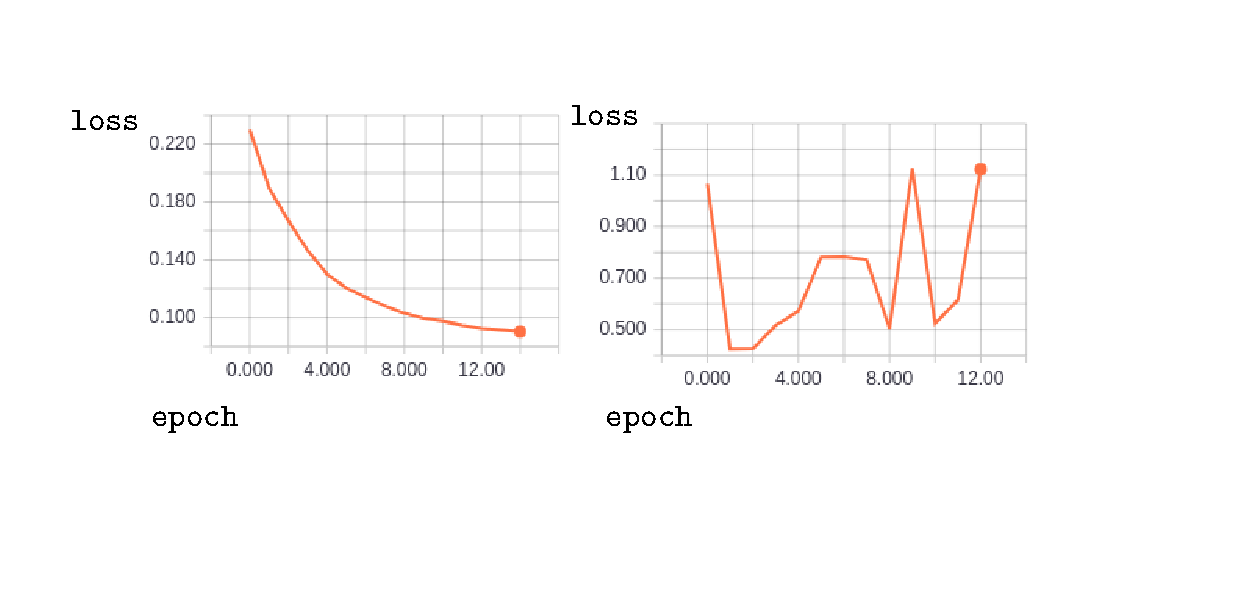
\includegraphics[width=\linewidth]{loss.pdf}
  \caption{Training of loss of two vanilla CNNS with similar hyperparameters}
  \label{fig:loss}
\end{figure}

\begin{figure}[h]
  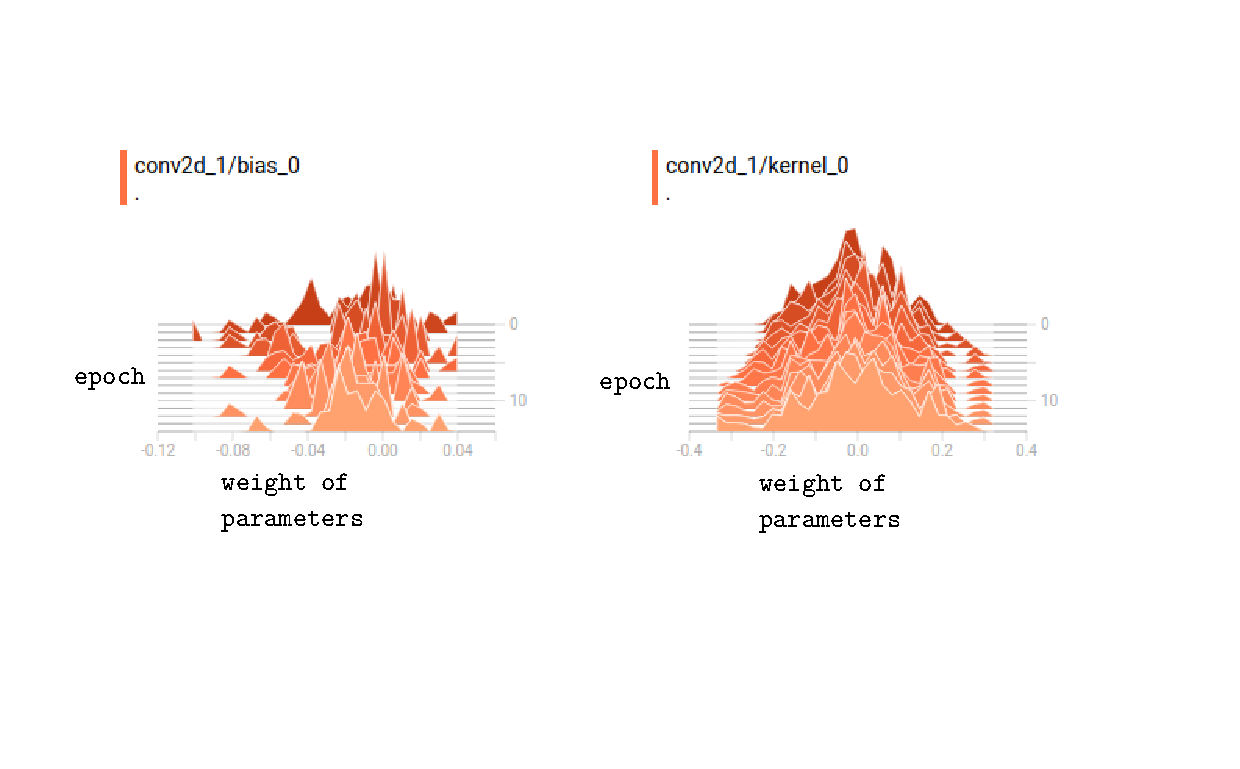
\includegraphics[width=\linewidth]{goodearlyweights.pdf}
  \caption{Convolutional layer bias and kernel parameter histograms for well performing model}
  \label{fig:goodearlyweights}
\end{figure}

\begin{figure}[h]
  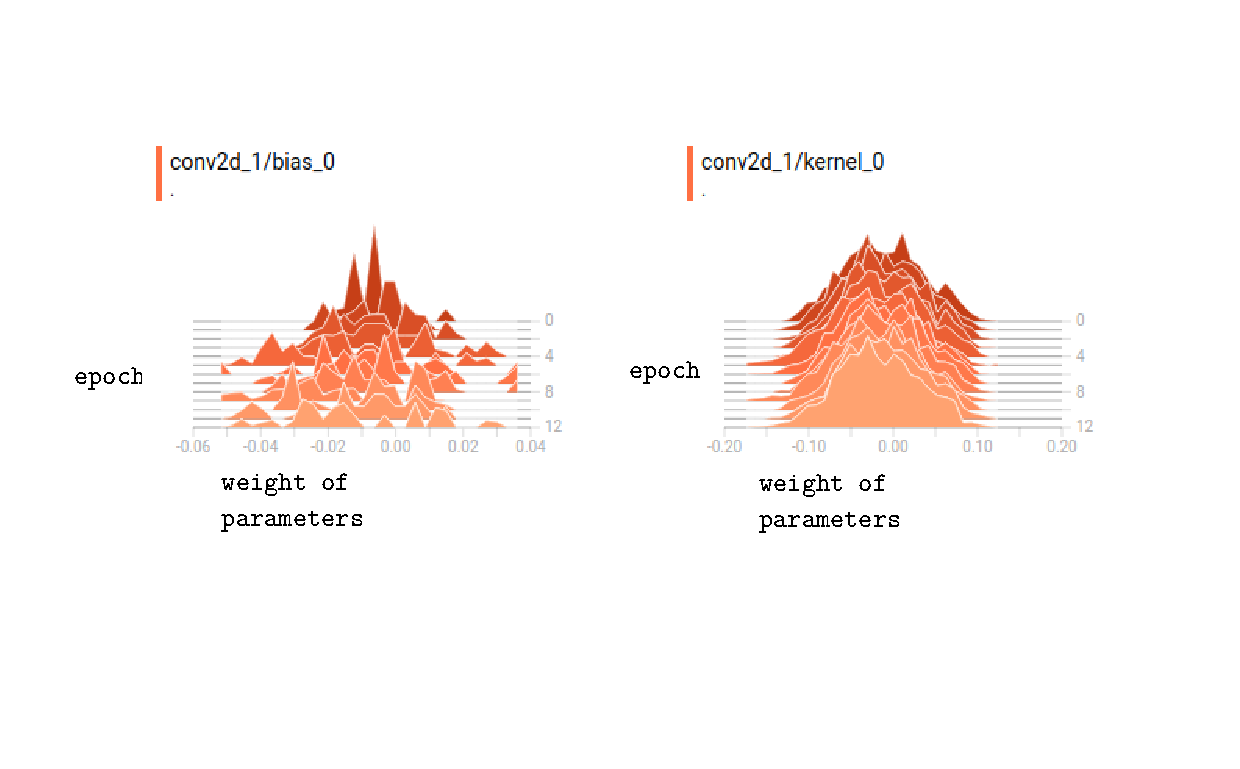
\includegraphics[width=\linewidth]{badearlyweights.pdf}
  \caption{Convolutional layer bias and kernel parameter histograms for poorly performing model}
  \label{fig:badearlyweights}
\end{figure}

\begin{figure}[h]
  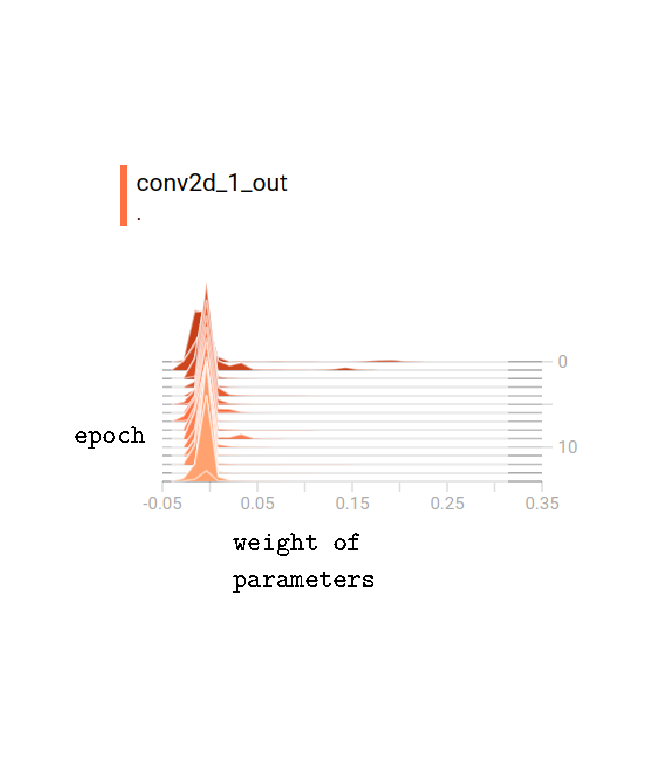
\includegraphics[scale=0.8]{goodearlyout.pdf}
  \caption{Convolutional layer output value histograms for well performing model}
  \label{fig:goodearlyout}
\end{figure}

\begin{figure}[h]
  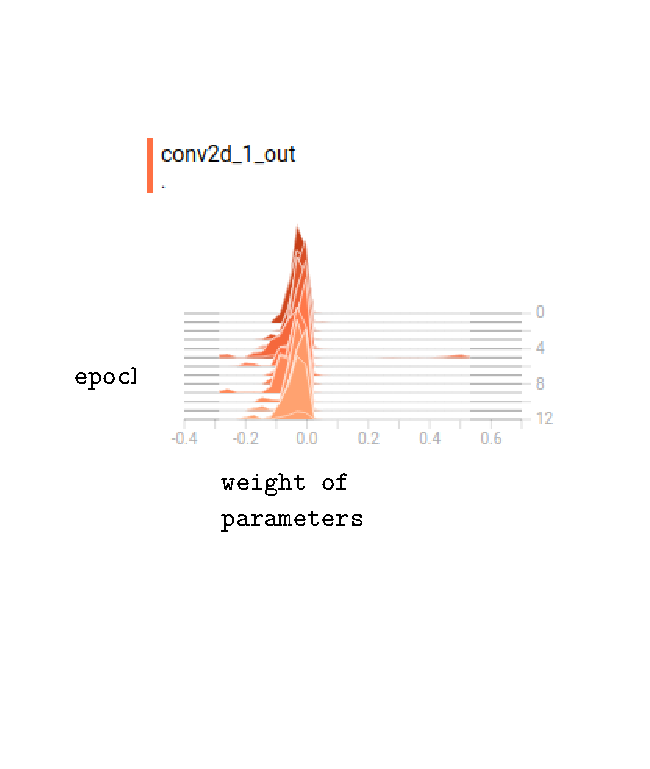
\includegraphics[scale=0.8]{badearlyout.pdf}
  \caption{Convolutional layer output value histograms for poorly performing model}
  \label{fig:badearlyout}
\end{figure}
has bad epoch

\begin{figure}[h]
  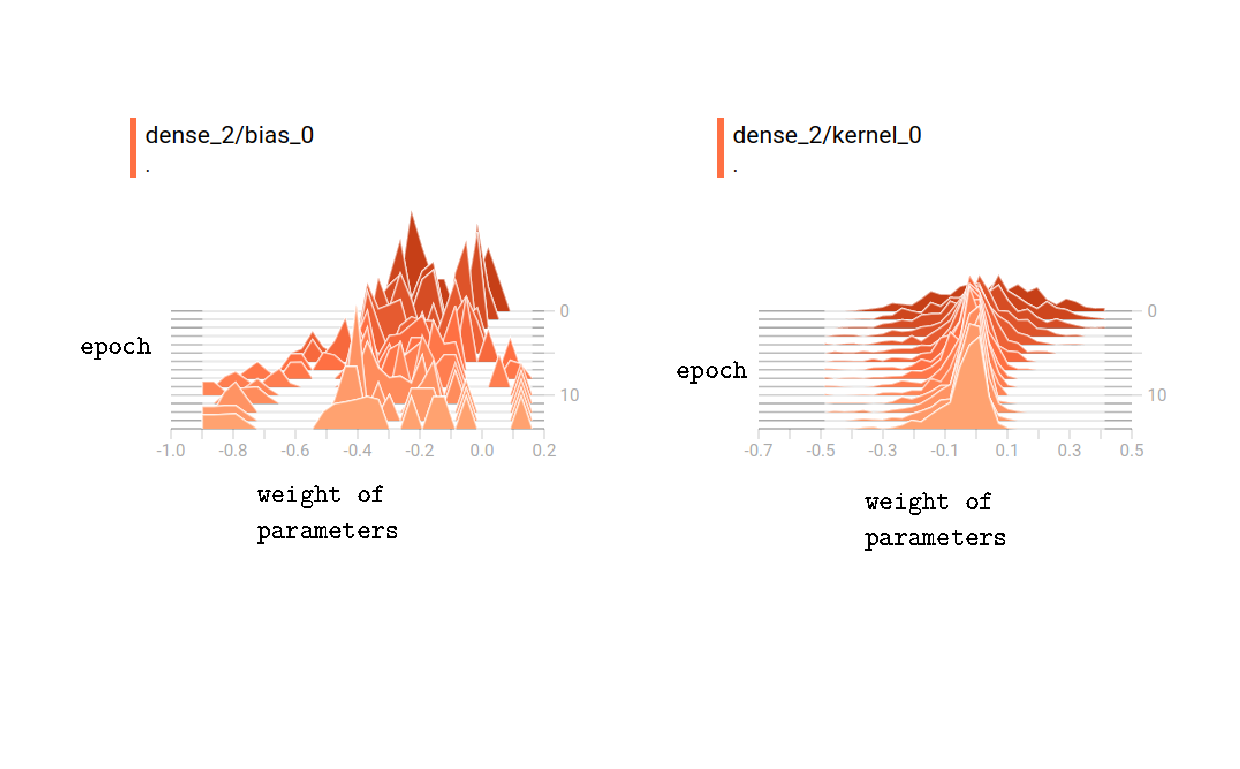
\includegraphics[width=\linewidth]{gooddense.pdf}
  \caption{Dense layer bias and kernel parameter histograms for well performing model}
  \label{fig:gooddenseweights}
\end{figure}

\begin{figure}[h]
  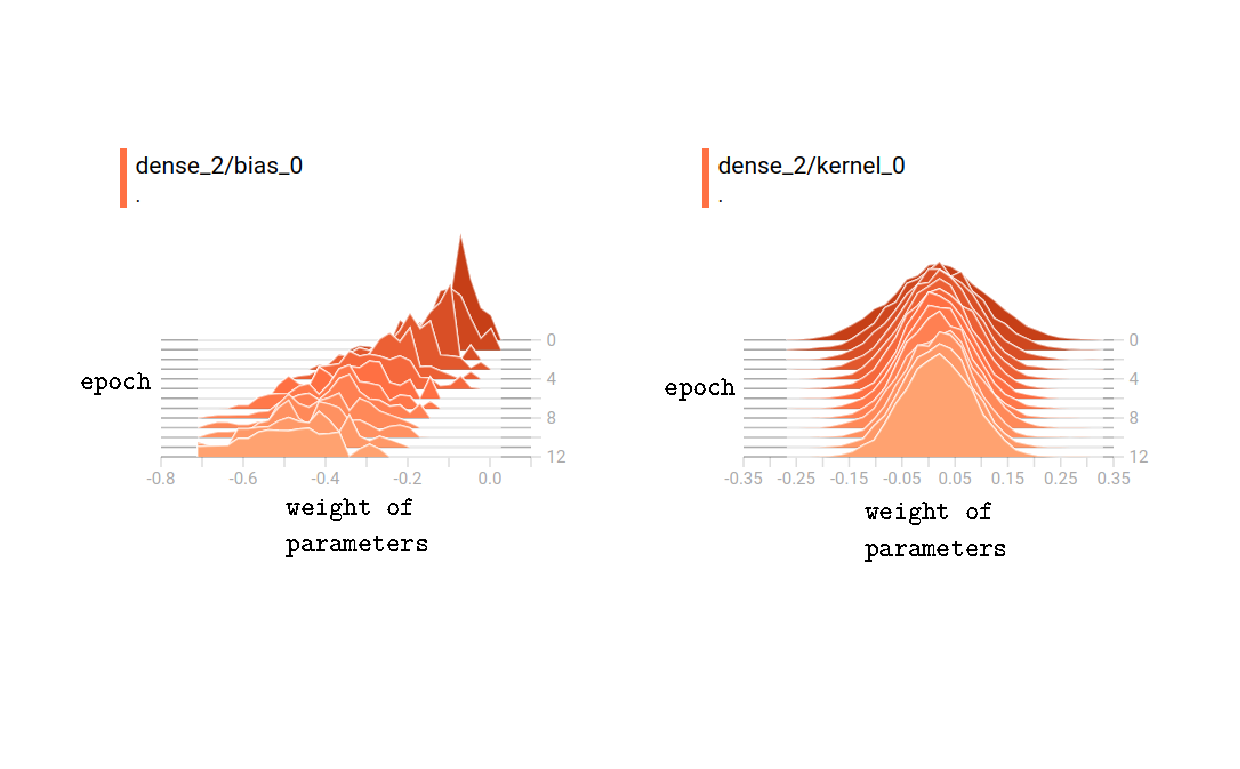
\includegraphics[width=\linewidth]{baddense.pdf}
  \caption{Dense layer bias and kernel parameter histograms for poorly performing model}
  \label{fig:baddenseweights}
\end{figure}

\begin{figure}[h]
  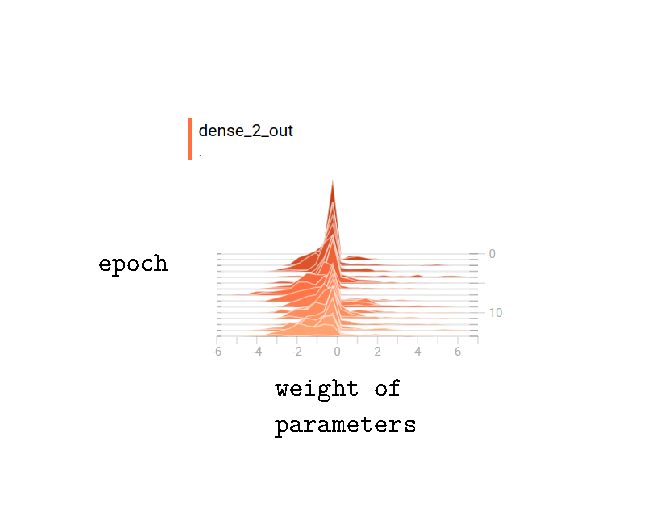
\includegraphics[scale=0.8]{gooddenseout.pdf}
  \caption{Dense layer output value histograms for well performing model}
  \label{fig:gooddenseout}
\end{figure}

\begin{figure}[h]
  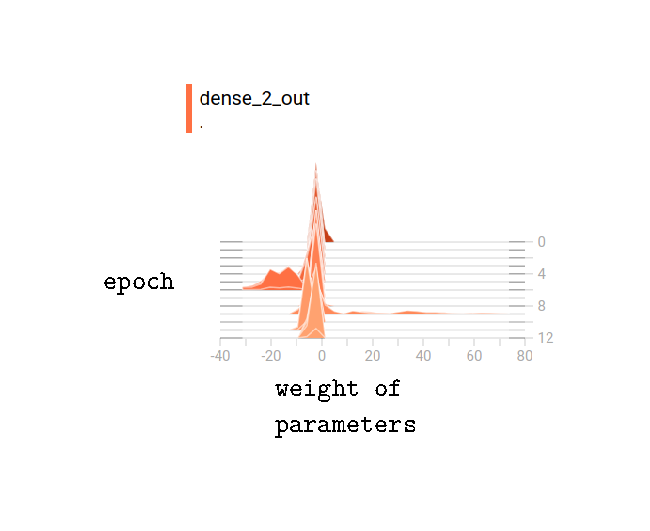
\includegraphics[scale=0.8]{baddenseout.pdf}
  \caption{Dense layer output value histograms for poorly performing model}
  \label{fig:baddenseout}
\end{figure}



\end{document}